\documentclass[11pt,a4paper]{article}
\usepackage[utf8]{inputenc}\usepackage[T1]{fontenc}\usepackage{mathptmx}\usepackage[scaled=0.9]{helvet}\usepackage{courier}
\usepackage[margin=2.3cm]{geometry}\usepackage{amsmath,amssymb}\usepackage{graphicx}
\usepackage{booktabs}\usepackage{listings}\usepackage{xcolor}\usepackage{fancyhdr}
\usepackage[hidelinks]{hyperref}\usepackage{caption}\usepackage{tikz}\usepackage{tabularx}\usepackage[section]{placeins}
\usetikzlibrary{positioning,arrows.meta}
\renewcommand{\contentsname}{Table des matières}
\renewcommand{\figurename}{Figure}\renewcommand{\tablename}{Tableau}
\pagestyle{fancy}\fancyhf{}
\lhead{\small Blombou -- Bouaboud -- Nanda -- Sissoko -- Ziani}\rhead{\small SIT213 -- Rapport Étapes 3 à 5}\cfoot{\thepage}
\lstset{language=Java,basicstyle=\ttfamily\small,columns=fullflexible,breaklines=true,frame=single,backgroundcolor=\color{gray!6},
  keywordstyle=\color{blue!60!black}\bfseries,commentstyle=\color{green!40!black}\itshape,
  literate={é}{{\'e}}1{è}{{\`e}}1{à}{{\`a}}1{É}{{\'E}}1{ê}{{\^e}}1{ù}{{\`u}}1{ç}{{\c{c}}}1}
\newcommand{\EbNo}{E_b/N_0}
\newcommand{\cls}[1]{\texttt{#1}}
\sloppy\setlength{\parskip}{4pt}\setlength{\parindent}{0pt}
\renewcommand{\partname}{Partie}
\begin{document}
\begin{titlepage}\centering
{\large IMT Atlantique -- FIP2A\\ Module SIT213\par}\vspace{3cm}
{\LARGE\bfseries Simulation d'une chaîne de transmission numérique\par}\vspace{0.6cm}
{\Large Rapport -- Étapes 3 à 5\\[4pt]\normalsize Canal gaussien, trajets multiples, récepteur à filtre adapté et codage de canal\par}\vspace{2.5cm}
\begin{tabular}{rl}
Groupe : & B4 -- FIP2A\\[4pt]
Auteurs : & BLOMBOU Ethan\\ & BOUABOUD Anis-Melwan\\ & NANDA Laurent\\ & SISSOKO Mohamed Djoncounda\\ & ZIANI Mohamed Amine\\[4pt]
Date : & Septembre 2026
\end{tabular}\vfill
\end{titlepage}
\tableofcontents\newpage

\section*{Organisation du rapport}
Ce rapport est cumulatif. La \textbf{partie~I} reprend sans modification le rapport de l'étape 3 (canal à bruit blanc additif gaussien). La \textbf{partie~II} présente l'étape 4 : le canal à trajets multiples et le récepteur à filtre adapté, qui lève la principale limite relevée à l'étape 3. La \textbf{partie~III} présente l'étape 5 : le codage de canal, puis un bilan des performances du simulateur et une conclusion générale. Chaque partie suit le même plan : objectifs, prévisions, réalisation, résultats, confrontation aux prévisions, tests.

\part{Étape 3 -- Canal à bruit blanc additif gaussien}
\section{Objectifs de l'étape 3}
L'étape 3 remplace le canal analogique parfait de l'étape 2 par un canal à \textbf{bruit blanc additif gaussien} (BBAG, ou AWGN). Le signal émis n'arrive plus intact au récepteur : des erreurs de décision apparaissent et le taux d'erreur binaire (TEB) devient non nul. L'objectif est donc de :
\begin{itemize}
  \item modéliser le canal $r(n) = s(n) + b(n)$ avec $b(n)\sim\mathcal N(0,\sigma_b^2)$ ;
  \item régler $\sigma_b^2$ à partir du rapport signal à bruit par bit $\EbNo$ fourni en paramètre ;
  \item vérifier que le bruit généré est bien gaussien ;
  \item tracer le TEB en fonction de $\EbNo$ et le confronter aux prévisions théoriques.
\end{itemize}

\section{Chaîne implémentée}
\begin{figure}[htbp]\centering
\resizebox{\linewidth}{!}{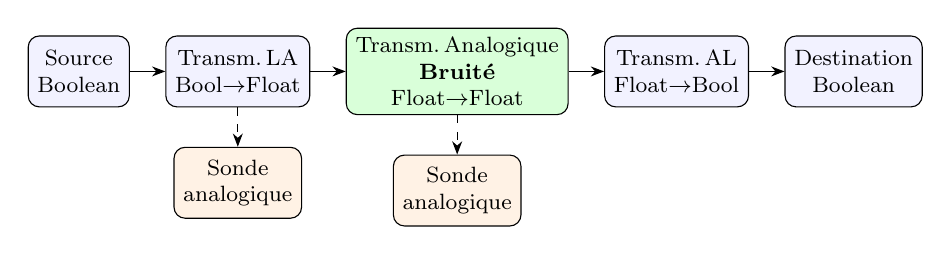
\begin{tikzpicture}[node distance=0.45cm,b/.style={draw,rounded corners,align=center,font=\footnotesize,minimum height=0.9cm,fill=blue!5},>=Stealth]
\node[b] (s) {Source\\Boolean};
\node[b,right=of s] (e) {Transm.\,LA\\Bool$\to$Float};
\node[b,right=of e,fill=green!15] (c) {Transm.\,Analogique\\\textbf{Bruité}\\Float$\to$Float};
\node[b,right=of c] (r) {Transm.\,AL\\Float$\to$Bool};
\node[b,right=of r] (d) {Destination\\Boolean};
\draw[->] (s)--(e); \draw[->] (e)--(c); \draw[->] (c)--(r); \draw[->] (r)--(d);
\node[b,below=0.5cm of e,fill=orange!10] (s1) {Sonde\\analogique}; \draw[->,dashed] (e)--(s1);
\node[b,below=0.5cm of c,fill=orange!10] (s2) {Sonde\\analogique}; \draw[->,dashed] (c)--(s2);
\end{tikzpicture}}
\caption{Chaîne de l'étape 3 -- seul le canal (en vert) change par rapport à l'étape 2.}
\end{figure}
L'architecture en composants connectables mise en place aux étapes 1 et 2 a permis d'introduire le bruit sans modifier ni l'émetteur (\texttt{TransmetteurLogiqueAnalogique}) ni le récepteur (\texttt{TransmetteurAnalogiqueLogique}) : le simulateur instancie simplement un \texttt{TransmetteurAnalogiqueBruite} à la place du \texttt{TransmetteurAnalogiqueParfait} lorsque l'option \texttt{-snrpb} est présente.

\section{Prévisions avant simulation}
\subsection{Paramètres pertinents}
\begin{center}\begin{tabular}{lll}\toprule
Paramètre & Option & Rôle\\\midrule
Rapport $\EbNo$ (dB) & \texttt{-snrpb} & fixe la puissance du bruit\\
Forme d'onde & \texttt{-form} & NRZ, NRZT ou RZ\\
Nombre d'échantillons par bit $N$ & \texttt{-nbEch} & intervient dans le calcul de $\sigma_b^2$\\
Amplitudes $A_{\min}, A_{\max}$ & \texttt{-ampl} & fixent la puissance $P_s$ et le seuil\\
Longueur du message & \texttt{-mess} & précision statistique du TEB\\
Semence & \texttt{-seed} & reproductibilité (message et bruit)\\\bottomrule
\end{tabular}\end{center}

\subsection{Résultats attendus}
\begin{itemize}
  \item Le TEB doit décroître de façon monotone quand $\EbNo$ augmente, et tendre vers $0{,}5$ quand $\EbNo\to-\infty$.
  \item Le TEB doit être indépendant de l'amplitude absolue du signal : multiplier $A_{\min}$ et $A_{\max}$ par un même facteur multiplie $P_s$, donc $\sigma_b$, dans le même rapport.
  \item Pour un récepteur optimal (filtre adapté), la théorie donne $\text{TEB} = Q\big(\sqrt{2\EbNo}\big)$ en NRZ antipodal et $Q\big(\sqrt{\EbNo}\big)$ pour un signal unipolaire (0, $A$), soit une pénalité de 3~dB pour l'unipolaire.
  \item Notre récepteur de l'étape 2 ne prend qu'\textbf{un seul échantillon par bit}. On s'attend donc à des performances inférieures à la borne optimale ; la section~\ref{sec:analyse} quantifie cet écart.
\end{itemize}

\section{Modélisation du canal gaussien}
\subsection{Réglage de la puissance du bruit}
D'après la séance 3, en notant $P_s$ la puissance moyenne du signal, $T$ la durée d'un bit, $F_e$ la fréquence d'échantillonnage et $N = TF_e$ le nombre d'échantillons par bit :
\[
E_b = P_s T,\qquad N_0 = \frac{2\sigma_b^2}{F_e}
\quad\Longrightarrow\quad
\frac{E_b}{N_0} = \frac{P_s\,N}{2\sigma_b^2}.
\]
On inverse cette relation pour obtenir la variance du bruit à appliquer :
\[
\boxed{\sigma_b^2 = \frac{P_s\,N}{2\cdot 10^{(\EbNo)_{\text{dB}}/10}}}
\]
La puissance $P_s$ est estimée directement sur le signal reçu par le canal, $P_s = \frac1K\sum_{n=1}^{K}s^2(n)$, ce qui la rend automatiquement correcte quelle que soit la forme d'onde et les amplitudes choisies.

\subsection{Génération du bruit}
Chaque échantillon de bruit est obtenu à partir de deux tirages uniformes indépendants $a_1, a_2\sim\mathcal U[0,1[$ (transformation de Box--Muller donnée en cours) :
\[ b(n) = \sigma_b\sqrt{-2\ln\big(1-a_1(n)\big)}\,\cos\big(2\pi a_2(n)\big). \]
L'utilisation de $1-a_1$ plutôt que $a_1$ évite le calcul de $\ln 0$, puisque \texttt{nextDouble()} peut renvoyer exactement 0.

\subsection{Classe \texttt{TransmetteurAnalogiqueBruite}}
\begin{itemize}
  \item Hérite de \texttt{Transmetteur<Float, Float>}.
  \item Constructeur \texttt{(int nbEch, float ebN0Db, Integer seed)} : le générateur \texttt{java.util.Random} est initialisé avec la semence si l'option \texttt{-seed} est fournie, ce qui permet de rejouer une simulation à l'identique.
  \item \texttt{emettre()} : calcule $P_s$, en déduit $\sigma_b$, ajoute un échantillon de bruit à chaque échantillon du signal puis transmet le résultat aux destinations connectées. Un message vide est retransmis tel quel.
\end{itemize}

\subsection{Nouvelle option du simulateur}
\begin{center}\begin{tabular}{ll}\toprule Option & Description\\\midrule
\texttt{-snrpb s} & canal bruité, $\EbNo = s$ dB (flottant, peut être négatif) ; active le mode analogique\\\bottomrule\end{tabular}\end{center}
Sans cette option, le canal reste parfait et le comportement des étapes 1 et 2 est inchangé. Le nom de l'option est celui imposé par la commande unique.

\subsection{Mise en conformité de l'analyse des arguments}
À l'occasion de cette étape, l'analyse des arguments a été alignée sur la commande unique : l'option \texttt{-ampl min max} lève désormais une \texttt{ArgumentsException} si $\text{min} \geq \text{max}$ (auparavant, \texttt{-ampl 1 0} était accepté et produisait un TEB de 1). Nous conservons en revanche un minimum de 10 échantillons par bit pour \texttt{-nbEch} : en dessous, le tiers central du RZ et la rampe du NRZT tiennent sur 0 ou 1 échantillon et la forme d'onde n'est plus correctement représentée. Ce choix est documenté dans le \texttt{README}.

\section{Validation du générateur de bruit}
Pour vérifier le générateur (remarque de la séance 3), on a envoyé dans le canal un signal constant égal à 1 ($P_s = 1$) sur 500\,000 échantillons avec $N = 30$ et $\EbNo = 10$~dB, puis soustrait le signal pour isoler le bruit.
\begin{center}\begin{tabular}{lcc}\toprule & Attendu & Mesuré\\\midrule
Moyenne & 0 & $5{,}6\times10^{-4}$\\
Écart-type $\sigma_b$ & $\sqrt{30/(2\cdot10)} = 1{,}2247$ & $1{,}2247$\\\bottomrule\end{tabular}\end{center}
\begin{figure}[htbp]\centering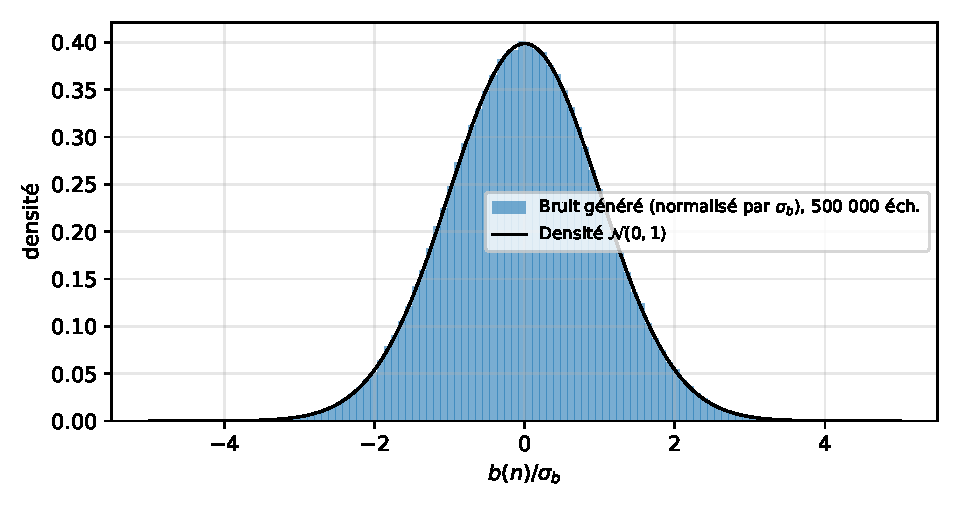
\includegraphics[width=0.8\linewidth]{../etape3/figures/fig_histo.pdf}
\caption{Histogramme du bruit généré comparé à la densité gaussienne centrée réduite.}\end{figure}
L'histogramme se superpose à la densité $\mathcal N(0,1)$ et l'écart-type mesuré coïncide avec la valeur calculée à $10^{-4}$ près : le générateur et le réglage de $\sigma_b$ sont validés.

\section{Résultats}
\subsection{Visualisation des signaux}
\begin{figure}[htbp]\centering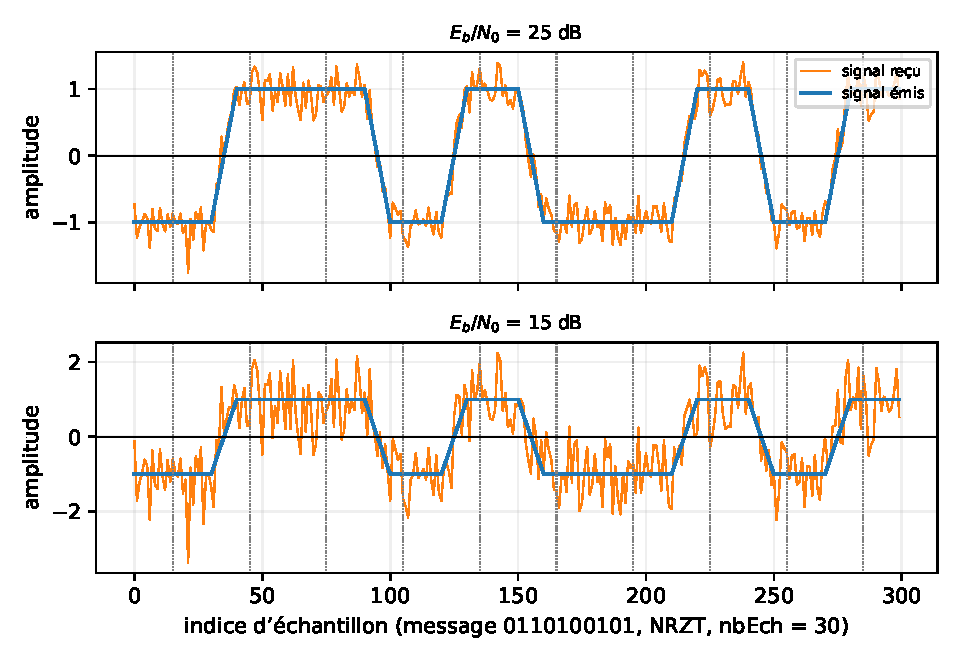
\includegraphics[width=0.88\linewidth]{../etape3/figures/fig_signal.pdf}
\caption{Signal NRZT émis et reçu pour deux valeurs de $\EbNo$. Les pointillés marquent l'échantillon central sur lequel le récepteur prend sa décision.}\end{figure}
Avec $N = 30$, même à $\EbNo = 25$~dB le bruit est bien visible sur chaque échantillon. À 15~dB, sa dispersion est du même ordre que l'amplitude du signal : un échantillon isolé peut franchir le seuil et provoquer une erreur de décision.

\subsection{TEB en fonction de $\EbNo$}
Les courbes ont été obtenues avec 200\,000 bits par point ($N = 30$), ce qui permet de mesurer des TEB jusqu'à environ $10^{-5}$. Les points à TEB nul ne sont pas représentés.
\begin{figure}[htbp]\centering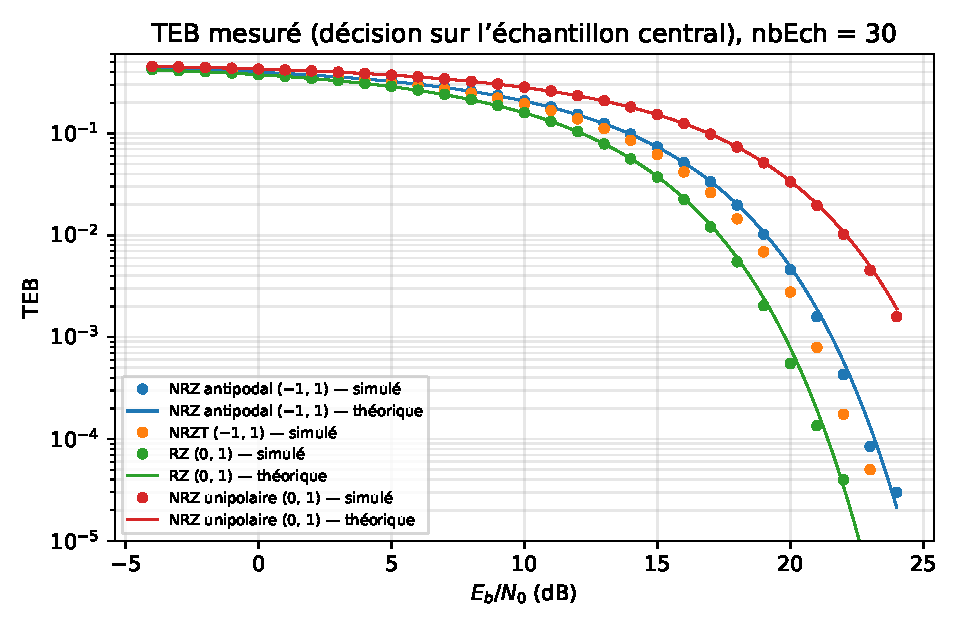
\includegraphics[width=0.9\linewidth]{../etape3/figures/fig_teb.pdf}
\caption{TEB simulé par notre chaîne (points) et TEB théorique pour une décision sur un échantillon (traits).}\label{fig:teb}\end{figure}

Quelques exécutions du simulateur en ligne de commande (100\,000 bits, $N = 30$) :
\begin{center}\footnotesize\begin{tabular}{lc}\toprule Commande & TEB\\\midrule
\texttt{-mess 100000 -form NRZ -ampl -1 1 -snrpb 8 -seed 1} & 0,259\\
\texttt{-mess 100000 -form NRZ -ampl -1 1 -snrpb 20 -seed 1} & $5{,}1\times10^{-3}$\\
\texttt{-mess 100000 -form NRZT -ampl -1 1 -snrpb 20 -seed 1} & $3{,}3\times10^{-3}$\\
\texttt{-mess 100000 -form RZ -snrpb 20 -seed 1} & $9{,}8\times10^{-4}$\\
\texttt{-mess 100000 -form NRZ -ampl -1 1 -snrpb 30 -seed 1} & 0\\\bottomrule\end{tabular}\end{center}
Deux exécutions avec la même semence donnent exactement le même TEB, ce qui confirme la reproductibilité.

\section{Confrontation aux prévisions}\label{sec:analyse}
\subsection{Ce qui est conforme}
Le TEB décroît bien de façon monotone avec $\EbNo$ et tend vers 0,5 aux faibles rapports. Il ne dépend pas de l'amplitude absolue, conformément à la normalisation par $P_s$.

\subsection{Écart par rapport à la borne optimale}
En revanche, les TEB mesurés sont très supérieurs à la prévision $Q(\sqrt{2\EbNo})$ : à 8~dB, on attendait environ $2\times10^{-4}$ en NRZ antipodal et l'on mesure 0,26. L'écart vient du récepteur, pas du canal.

Le récepteur décide à partir d'\textbf{un seul} échantillon, dont le rapport signal à bruit vaut, pour un NRZ antipodal ($\pm A$, $P_s = A^2$) :
\[ \frac{A^2}{\sigma_b^2} = \frac{A^2\cdot 2\,\EbNo}{A^2 N} = \frac{2}{N}\frac{E_b}{N_0}
\quad\Longrightarrow\quad \text{TEB} = Q\!\left(\sqrt{\tfrac{2}{N}\tfrac{E_b}{N_0}}\right). \]
L'énergie du bit est répartie sur $N$ échantillons, mais le récepteur n'en exploite qu'un : il perd un facteur $N$, soit $10\log_{10}30\approx 14{,}8$~dB. Le même raisonnement donne :
\begin{center}\begin{tabular}{lccc}\toprule
Forme & $P_s$ & Distance au seuil & TEB (1 échantillon)\\\midrule
NRZ antipodal $(-A, A)$ & $A^2$ & $A$ & $Q\big(\sqrt{2\EbNo/N}\big)$\\
NRZ unipolaire $(0, A)$ & $A^2/2$ & $A/2$ & $Q\big(\sqrt{\EbNo/N}\big)$\\
RZ $(0, A)$ & $A^2/6$ & $A/2$ & $Q\big(\sqrt{3\EbNo/N}\big)$\\\bottomrule\end{tabular}\end{center}
Ces expressions (traits de la figure~\ref{fig:teb}) se superposent aux points simulés, ce qui valide à la fois le canal et notre compréhension du récepteur.

\subsection{Classement des formes d'onde}
\begin{itemize}
  \item \textbf{NRZ unipolaire vs antipodal} : 3~dB d'écart, comme prévu par la théorie.
  \item \textbf{NRZT} : légèrement meilleur que le NRZ (environ 0,5~dB). Les rampes réduisent la puissance moyenne ($P_s \approx 0{,}89\,A^2$), donc $\sigma_b$, alors que l'échantillon central reste sur le plateau à $\pm A$.
  \item \textbf{RZ} : meilleur que le NRZ antipodal avec ce récepteur (environ 1,8~dB), ce qui contredit l'intuition. C'est un artefact de la décision ponctuelle : le signal RZ est nul les deux tiers du temps, sa puissance moyenne est faible, et le bruit calibré sur $\EbNo$ l'est aussi, alors que l'échantillon central tombe précisément sur l'impulsion. Avec un récepteur optimal, le RZ unipolaire retrouve sa place, 3~dB derrière le NRZ antipodal.
\end{itemize}

\section{Piste d'amélioration : récepteur moyenneur}
Pour vérifier l'analyse précédente, nous avons testé hors du simulateur, à l'aide d'un banc de mesure réutilisant nos classes \texttt{SourceAleatoire}, \texttt{TransmetteurLogiqueAnalogique} et \texttt{TransmetteurAnalogiqueBruite}, une décision sur la \textbf{moyenne des échantillons} du temps bit (sur tout le bit en NRZ, sur le tiers central en RZ). Moyenner $M$ échantillons divise la variance du bruit par $M$ sans changer le niveau utile ; c'est l'équivalent discret du filtre adapté pour une impulsion rectangulaire.
\begin{figure}[htbp]\centering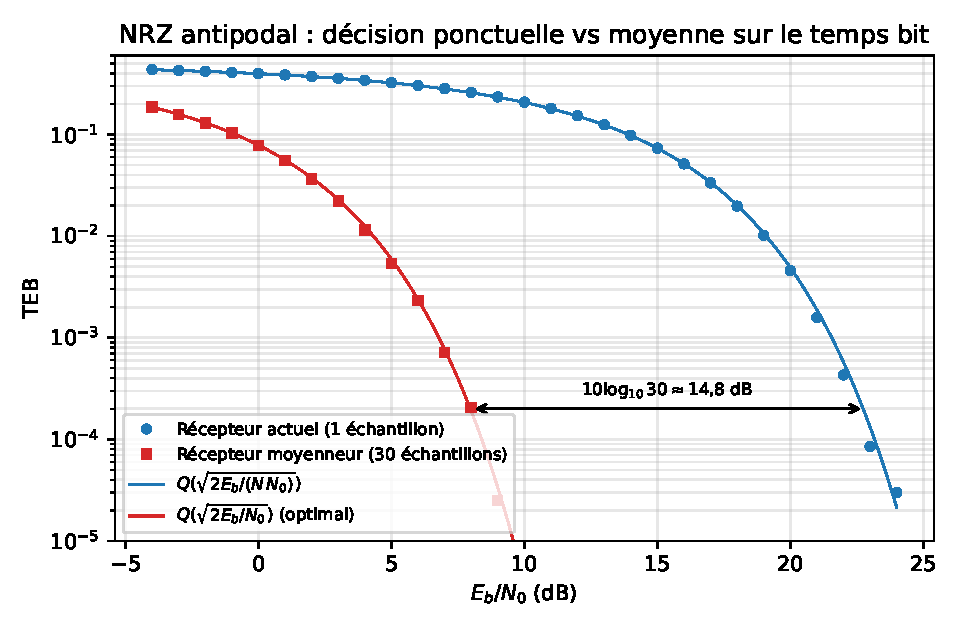
\includegraphics[width=0.85\linewidth]{../etape3/figures/fig_moy.pdf}
\caption{NRZ antipodal : récepteur actuel et récepteur moyenneur, 200\,000 bits par point.}\end{figure}
Le récepteur moyenneur atteint la borne $Q(\sqrt{2\EbNo})$ (TEB mesuré de $2{,}05\times10^{-4}$ à 8~dB pour $1{,}9\times10^{-4}$ attendu), soit un gain de 14,8~dB. En RZ, moyenner sur le tiers central donne $Q(\sqrt{\EbNo})$ ($5{,}7\times10^{-3}$ mesuré à 8~dB pour $6\times10^{-3}$ attendu). Ce récepteur n'est pas encore intégré dans \texttt{TransmetteurAnalogiqueLogique} ; il le sera dans une prochaine version, avec une option permettant de conserver la décision ponctuelle pour comparaison.

\section{Tests}
\subsection{Tests automatiques (\texttt{runTests})}
Neuf tests ont été ajoutés pour l'étape 3 : cinq exécutions nominales ($\EbNo$ élevé et faible, chaîne NRZT complète, \texttt{-snrpb} seul, performance sur 10\,000 bits limitée à 10~s) et quatre tests d'erreur sur les nouveaux contrôles d'arguments.
\begin{lstlisting}[language={}]
Test 10 : Bruit (Eb/N0 élevé, peu d'erreurs) ... OK
Test 11 : Bruit (Eb/N0 faible, beaucoup d'erreurs) ... OK
Test 12 : Bruit complet (NRZT + ampl + snrpb) ... OK
Test 13 : Bruit seul (-snrpb active le mode analogique) ... OK
Test 14 : Performance (message aléatoire de 10000 bits) ... OK
Test 19 : Erreur (ampl min > max) ... OK
Test 20 : Erreur (ampl min = max) ... OK
Test 21 : Erreur (snrpb non flottant) ... OK
Test 22 : Erreur (snrpb sans valeur) ... OK
\end{lstlisting}

\subsection{Tests unitaires JUnit}
Six tests ont été ajoutés à \texttt{SimulateurTest} : refus de \texttt{-ampl} avec $\text{min} > \text{max}$ et $\text{min} = \text{max}$, TEB non nul à 0~dB, TEB nul à 40~dB, refus d'une valeur non flottante pour \texttt{-snrpb} et refus de l'ancienne option \texttt{-ebn0}. L'ensemble de la suite passe : 75 tests sur 75.

\subsection{Limites identifiées}
\begin{itemize}
  \item Ces tests vérifient que le simulateur s'exécute et affiche un TEB, pas la valeur du TEB. Un test de non-régression comparant le TEB mesuré à la valeur théorique, avec une tolérance, serait plus robuste.
  \item Avec \texttt{-seed}, la source et le canal sont initialisés avec la \textbf{même} semence. Les deux générateurs produisent alors des suites liées. Utiliser deux semences dérivées (par exemple \texttt{seed} et \texttt{seed + 1}) garantirait l'indépendance du message et du bruit.
\end{itemize}

\section{Conclusion}
Le canal à bruit blanc additif gaussien est fonctionnel et validé : le bruit généré est gaussien, centré, et son écart-type correspond exactement à la valeur déduite de $\EbNo$. Les TEB mesurés concordent avec la théorie pour le récepteur actuel, qui décide sur un seul échantillon par bit.

La confrontation aux prévisions met en évidence la principale limite de la chaîne : ce récepteur perd $10\log_{10}N\approx14{,}8$~dB par rapport à l'optimum. Un récepteur moyenneur, testé sur banc, atteint la borne théorique. Son intégration est la priorité avant l'étape 5b, qui cherchera à réduire le TEB par codage de canal : il serait incohérent de coder le canal avant d'avoir récupéré ces 15~dB à la réception.

\part{Étape 4 -- Canal à trajets multiples et récepteur à filtre adapté}
\section{Objectifs de l'étape 4}
L'énoncé de l'atelier découpe l'étape 4 en deux parties :
\begin{itemize}
  \item \textbf{4a} -- transmission non idéale avec un bruit « réel » : nous avons retenu les \textbf{trajets multiples}, décrits par la fiche de la séance 4. Le signal reçu est la somme du trajet direct et de copies retardées et atténuées :
  \[ r(n) = s(n) + \sum_{k=1}^{K} ar_k\, s(n - dt_k), \qquad K \le 5 ; \]
  \item \textbf{4b} -- les mêmes trajets multiples \textbf{plus} le bruit blanc gaussien de l'étape 3 : $r(n) = s(n) + \sum_k ar_k\,s(n-dt_k) + b(n)$.
\end{itemize}
Le rapport de l'étape 3 concluait par ailleurs que notre récepteur, qui décidait sur un seul échantillon par bit, perdait $10\log_{10}N \approx 14{,}8$~dB par rapport à l'optimum, et que l'intégration d'un récepteur optimal était la priorité avant le codage de canal. Cette étape réalise donc aussi le \textbf{récepteur à filtre adapté}. Les objectifs sont :
\begin{itemize}
  \item modéliser le canal à trajets multiples, avec ou sans bruit, et l'intégrer au simulateur via l'option \texttt{-ti} de la commande unique ;
  \item remplacer la décision sur l'échantillon central par un filtre adapté valable pour les trois formes d'onde ;
  \item mesurer le TEB dans chaque configuration et le confronter à une théorie exacte de la chaîne.
\end{itemize}

%======================================================================
\section{Chaîne implémentée}
\begin{figure}[htbp]\centering
\resizebox{\linewidth}{!}{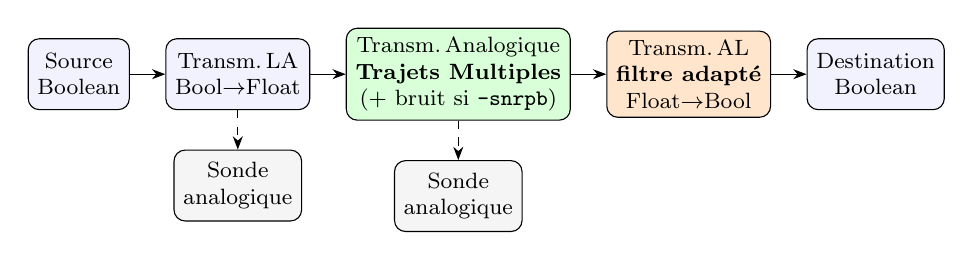
\begin{tikzpicture}[node distance=0.45cm,b/.style={draw,rounded corners,align=center,font=\footnotesize,minimum height=0.9cm,fill=blue!5},>=Stealth]
\node[b] (s) {Source\\Boolean};
\node[b,right=of s] (e) {Transm.\,LA\\Bool$\to$Float};
\node[b,right=of e,fill=green!15] (c) {Transm.\,Analogique\\\textbf{Trajets Multiples}\\(+ bruit si \texttt{-snrpb})};
\node[b,right=of c,fill=orange!20] (r) {Transm.\,AL\\\textbf{filtre adapté}\\Float$\to$Bool};
\node[b,right=of r] (d) {Destination\\Boolean};
\draw[->] (s)--(e); \draw[->] (e)--(c); \draw[->] (c)--(r); \draw[->] (r)--(d);
\node[b,below=0.5cm of e,fill=gray!8] (s1) {Sonde\\analogique}; \draw[->,dashed] (e)--(s1);
\node[b,below=0.5cm of c,fill=gray!8] (s2) {Sonde\\analogique}; \draw[->,dashed] (c)--(s2);
\end{tikzpicture}}
\caption{Chaîne de l'étape 4. En vert, le nouveau canal ; en orange, le récepteur modifié.}
\end{figure}
Le simulateur choisit le canal selon les options présentes :
\begin{center}\begin{tabular}{lll}\toprule
Options & Canal instancié & Perturbation\\\midrule
aucune & \cls{TransmetteurAnalogiqueParfait} & aucune\\
\texttt{-snrpb s} & \cls{TransmetteurAnalogiqueBruite} & bruit gaussien (étape 3)\\
\texttt{-ti dt ar ...} & \cls{TransmetteurAnalogiqueTrajetsMultiples} & échos seuls (4a)\\
\texttt{-ti dt ar ... -snrpb s} & \cls{TransmetteurAnalogiqueTrajetsMultiples} & échos puis bruit (4b)\\\bottomrule
\end{tabular}\end{center}
Le récepteur à filtre adapté est utilisé dans tous les cas analogiques.

%======================================================================
\section{Récapitulatif des modifications depuis l'étape 3}
\begin{center}\small\begin{tabularx}{\linewidth}{>{\raggedright\arraybackslash}p{4.6cm}X}\toprule
Élément & Modification\\\midrule
\texttt{TransmetteurAnalogique}\newline\texttt{TrajetsMultiples} & \textbf{Nouvelle classe.} Canal à trajets multiples, bruité ou non. Hérite de \cls{TransmetteurAnalogiqueBruite} (section~\ref{sec:heritage}).\\
\texttt{TransmetteurAnalogique}\newline\texttt{Bruite} & Le calcul du signal auquel on ajoute le bruit est isolé dans une méthode protégée \texttt{signalAvantBruit()}, que la sous-classe redéfinit. Comportement inchangé pour le canal gaussien seul.\\
\texttt{TransmetteurAnalogique}\newline\texttt{Logique} & \textbf{Récepteur à filtre adapté} : corrélation de tout le temps bit avec $g = s_1 - s_0$ au lieu d'un seuil sur l'échantillon central (section~\ref{sec:filtre}). Le constructeur reçoit désormais la forme d'onde.\\
\texttt{TransmetteurLogique}\newline\texttt{Analogique} & La génération d'un bit est extraite dans \texttt{formeBit(...)}, partagée avec le récepteur. Signal émis inchangé.\\
\texttt{Simulateur} & Nouvelle option \texttt{-ti} ; sélection du canal ; Eb/N0 infini sans \texttt{-snrpb} ; forme d'onde transmise au récepteur.\\
\texttt{runTests} & Section « Étape 4 » : 3 exécutions nominales et 3 tests d'erreur sur \texttt{-ti} ; renumérotation des commentaires (28 tests).\\
Tests JUnit & 22 tests ajoutés, 1 supprimé (option \texttt{-ebn0} hors spécification) : 96 tests, tous réussis.\\
\texttt{genDeliverable}, \texttt{README} & Archive \texttt{etape4} ; documentation de \texttt{-ti} et du filtre adapté, exemples remesurés.\\
\texttt{rapport/etape4/} & Script \texttt{courbesTEB.py} (simulations et théorie exacte) et outil \texttt{ExportSignal.java} qui produisent toutes les figures de ce rapport.\\\bottomrule
\end{tabularx}\end{center}

%======================================================================
\section{Prévisions avant simulation}
\subsection{Paramètres pertinents}
\begin{center}\begin{tabular}{lll}\toprule
Paramètre & Option & Rôle\\\midrule
Retard $dt_k$ d'un trajet indirect (échantillons) & \texttt{-ti} & position de l'écho par rapport au bit\\
Amplitude relative $ar_k$ & \texttt{-ti} & force de l'écho\\
Nombre de trajets (1 à 5) & \texttt{-ti} & nombre de couples $dt\ ar$\\
Rapport $\EbNo$ (dB) & \texttt{-snrpb} & bruit ajouté après les échos (4b)\\
Forme d'onde, $N$, amplitudes & \texttt{-form}, \texttt{-nbEch}, \texttt{-ampl} & forme du filtre adapté et du seuil\\\bottomrule
\end{tabular}\end{center}

\subsection{Résultats attendus}
\begin{itemize}
  \item \textbf{Filtre adapté.} Le TEB doit rejoindre la borne optimale : $Q\big(\sqrt{2\EbNo}\big)$ en NRZ antipodal et $Q\big(\sqrt{\EbNo}\big)$ en unipolaire, soit un gain de $10\log_{10}N \approx 14{,}8$~dB sur l'étape 3.
  \item \textbf{Trajets multiples sans bruit (4a).} L'écho d'un bit « déborde » sur les bits suivants : c'est de l'interférence entre symboles (IES). Tant qu'elle ne fait pas franchir le seuil, le TEB reste nul ; au-delà, le TEB passe brusquement à une fraction fixe (les suites de bits défavorables). Un écho retardé d'un bit entier ($dt = N$) doit être le plus gênant.
  \item \textbf{Trajets multiples et bruit (4b).} Pour un même $\EbNo$, le TEB doit être plus élevé qu'en l'absence d'écho, et d'autant plus que $ar$ est grand.
\end{itemize}

%======================================================================
\section{Modélisation du canal à trajets multiples}
\subsection{Modèle discret}
Chaque trajet indirect $k$ est une copie du signal émis, décalée de $dt_k$ échantillons et multipliée par $ar_k$ :
\[ r(n) = s(n) + \sum_{k=1}^{K} ar_k\, s(n - dt_k) \quad (+\,b(n)\ \text{en 4b}), \qquad s(m) = 0 \text{ pour } m < 0. \]
Avant le début d'un écho ($n < dt_k$), rien n'est encore réfléchi. La longueur du signal est conservée : la queue de l'écho du dernier bit est tronquée, ce qui est sans effet sur la décision.

\subsection{Option \texttt{-ti} de la commande unique}
La commande unique impose la syntaxe \texttt{-ti dt ar [dt ar ...]} : le retard (entier) vient avant l'amplitude (flottant), jusqu'à 5 couples, sans indiquer leur nombre. L'analyse lit des couples tant que l'argument suivant est un entier :
\begin{lstlisting}
} else if (args[i].matches("-ti")) {
    // Syntaxe : -ti dt1 ar1 [dt2 ar2 ...] (5 couples au maximum)
    simulationAnalogique = true;
    canalTrajetsMultiples = true;
    while (i + 1 < args.length && args[i + 1].matches("-?[0-9]+")) {
        i++;  int dt = Integer.parseInt(args[i]);      // dt >= 0, sinon erreur
        i++;  amplitudes.add(Float.parseFloat(args[i])); // ar manquant ou non flottant : erreur
        retards.add(dt);
    }
    if (retards.isEmpty() || retards.size() > NB_TRAJETS_MAX) throw new ArgumentsException(...);
\end{lstlisting}
Les arguments invalides lèvent une \cls{ArgumentsException} : \texttt{-ti} sans couple, plus de 5 couples, \texttt{ar} manquant ou non numérique, \texttt{dt} négatif ou hors des entiers. Un \texttt{dt} négatif est refusé car il désignerait un écho arrivant \emph{avant} le trajet direct ; il provoquait de plus un accès hors du tableau. Comme \texttt{-form} ou \texttt{-snrpb}, \texttt{-ti} active la simulation analogique.

\subsection{Implémentation par héritage}\label{sec:heritage}
Un canal à trajets multiples bruité est un canal gaussien dans lequel on insère une étape avant l'ajout du bruit. Plutôt que de dupliquer le calcul du bruit, la nouvelle classe hérite de \cls{TransmetteurAnalogiqueBruite}, selon le patron « méthode modèle » :
\begin{center}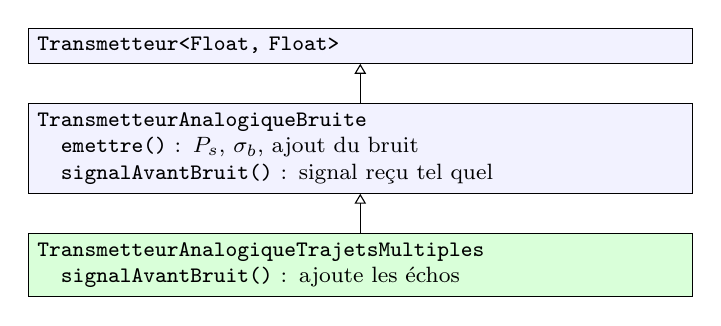
\begin{tikzpicture}[b/.style={draw,align=left,font=\footnotesize,fill=blue!5,text width=8.2cm},>=Stealth]
\node[b] (t) {\texttt{Transmetteur<Float, Float>}};
\node[b,below=0.5cm of t] (b) {\texttt{TransmetteurAnalogiqueBruite}\\\quad\texttt{emettre()} : $P_s$, $\sigma_b$, ajout du bruit\\\quad\texttt{signalAvantBruit()} : signal reçu tel quel};
\node[b,below=0.5cm of b,fill=green!15] (m) {\texttt{TransmetteurAnalogiqueTrajetsMultiples}\\\quad\texttt{signalAvantBruit()} : ajoute les échos};
\draw[-{Triangle[open]}] (b)--(t); \draw[-{Triangle[open]}] (m)--(b);
\end{tikzpicture}\end{center}
\begin{lstlisting}
// TransmetteurAnalogiqueBruite.emettre() (extrait simplifié)
float[] signal = signalAvantBruit();            // point d'extension
double ps = sommeCarres(signal) / n;            // puissance mesurée après les échos
double sigmaB2 = (ps * nbEch) / (2.0 * ebN0Lineaire);
for (int i = 0; i < n; i++)
    informationEmise.add((float) (signal[i] + genererBruitGaussien(sigmaB)));

// TransmetteurAnalogiqueTrajetsMultiples
@Override
protected float[] signalAvantBruit() {
    for (int i = 0; i < n; i++) {
        float valeur = informationRecue.iemeElement(i);
        for (int k = 0; k < retards.length; k++)
            if (i - retards[k] >= 0)
                valeur += amplitudes[k] * informationRecue.iemeElement(i - retards[k]);
        avecTrajets[i] = valeur;
    }
    return avecTrajets;
}
\end{lstlisting}
Conséquences :
\begin{itemize}
  \item la formule du bruit n'existe qu'à un seul endroit, ce qui garantit qu'un même \texttt{-snrpb} donne le même bruit dans les deux canaux ;
  \item conformément à la fiche de la séance 4, $P_s = \frac1N\sum s_{tj}^2$ est mesurée sur le signal \emph{avec échos} ;
  \item sans \texttt{-snrpb}, le simulateur transmet $\EbNo = +\infty$ : on obtient alors $\sigma_b = 0$ et aucun bruit n'est ajouté (étape 4a), sans aucun cas particulier dans le code.
\end{itemize}

\subsection{Défauts corrigés dans la première version}
La première version du canal (commit « Ajout du signal bruité ») a été relue et confrontée à la commande unique. Cinq défauts ont été corrigés :
\begin{center}\small\begin{tabularx}{\linewidth}{>{\raggedright\arraybackslash}p{4.3cm}Xl}\toprule
Défaut & Effet mesuré & Correction\\\midrule
Option \texttt{-trajets n ar dt ...} & refus des commandes de l'enseignant (\texttt{-ti}) & syntaxe \texttt{-ti dt ar}\\
Condition \texttt{canalBruite} testée deux fois & \texttt{-trajets} sans effet & branchement corrigé\\
$\EbNo$ par défaut à 0~dB & écho $dt = N$, $ar = 0{,}5$, sans \texttt{-snrpb} (NRZ $\pm1$, $N = 10$) : TEB $0{,}150$ au lieu de 0 & $\EbNo = +\infty$\\
Facteur $N$ oublié dans $\sigma_b^2$ (copie de la formule) & bruit 30 fois trop faible : écho nul, 0~dB (NRZ $0/1$), TEB $0{,}158$ au lieu de $0{,}428$ & héritage\\
Retard négatif accepté & accès hors du tableau & refusé\\\bottomrule
\end{tabularx}\end{center}
Le troisième défaut rendait un test JUnit trompeur : « TEB non nul avec \texttt{-trajets} sans \texttt{-snrpb} » ne réussissait que grâce au bruit caché. Il a été remplacé par deux tests, l'un avec des échos réellement destructeurs, l'autre vérifiant qu'un écho faible sans bruit donne un TEB nul.

%======================================================================
\section{Récepteur à filtre adapté}\label{sec:filtre}
\subsection{Principe}
Pour une impulsion $p(t)$ de durée $T$ reçue dans un bruit blanc gaussien, le filtre linéaire qui maximise le rapport signal à bruit à l'instant de décision est le \textbf{filtre adapté}, de réponse impulsionnelle $h(t) = p(T-t)$ : l'impulsion retournée dans le temps et décalée pour être causale~[1]. Échantillonnée en $t = T$, sa sortie est une \textbf{corrélation} :
\[ y(T) = \int r(\tau)\,h(T-\tau)\,d\tau = \int_0^T r(\tau)\,p(\tau)\,d\tau . \]
Le signal utile s'additionne de façon cohérente sur tout le bit, alors que le bruit, indépendant d'un échantillon à l'autre, se moyenne. C'est précisément ce que ne faisait pas le récepteur de l'étape 3, qui n'utilisait qu'un échantillon sur $N$.

\subsection{Une règle de décision unique pour les trois formes d'onde}
Notons $s_1$ et $s_0$ les $N$ échantillons d'un bit 1 et d'un bit 0, et $r$ les échantillons reçus pendant un bit. Avec un bruit gaussien, la décision optimale choisit le symbole le plus proche :
\[ \|r - s_1\|^2 < \|r - s_0\|^2 \iff \underbrace{\sum_{k=0}^{N-1} r[k]\, g[k]}_{y} > \underbrace{\frac{\|s_1\|^2 - \|s_0\|^2}{2}}_{\text{seuil}}, \qquad g = s_1 - s_0 . \]
C'est un filtre adapté à la \emph{différence} $g$ des deux symboles. La forme d'onde n'apparaît que dans $g$ : la même formule convient à NRZ, NRZT et RZ, et le seuil s'en déduit automatiquement (figure~\ref{fig:filtres}) :
\begin{itemize}
  \item \textbf{NRZ} : $g$ est constant, $y$ est la somme des échantillons du bit ; ramené à une moyenne, le seuil vaut $(A_{\min}+A_{\max})/2$ comme à l'étape 3 ;
  \item \textbf{RZ} : $g$ est nul hors du tiers central, qui ne contient que du bruit ; le filtre l'ignore ;
  \item \textbf{NRZT} : les échantillons des rampes, moins fiables, reçoivent un poids plus faible.
\end{itemize}
\begin{figure}[htbp]\centering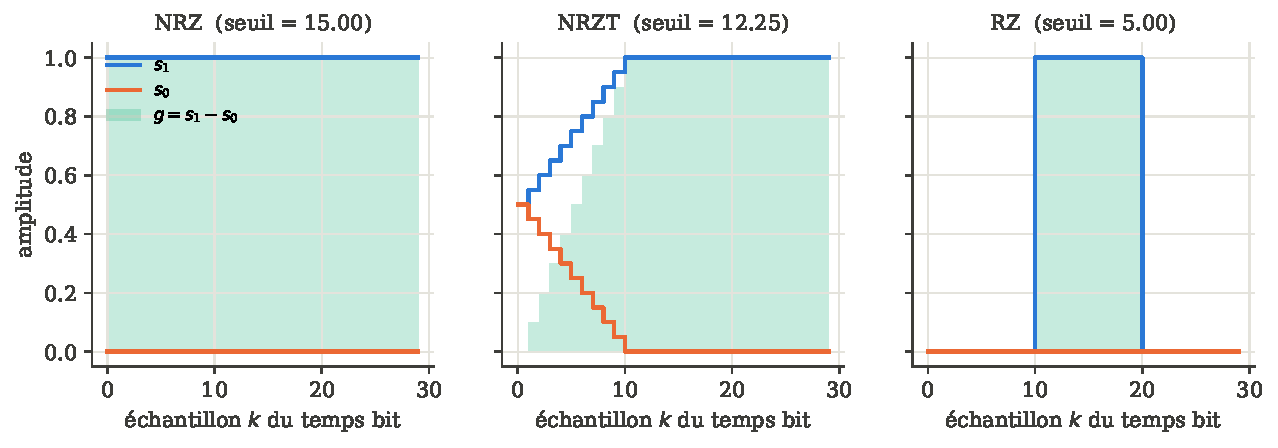
\includegraphics[width=\linewidth]{../etape4/figures/fig_filtres.pdf}
\caption{Formes de référence $s_1$, $s_0$ et filtre $g = s_1 - s_0$ pour $N = 30$ et les amplitudes $(0, 1)$. Le seuil est exprimé en unités de la somme $y$.}\label{fig:filtres}\end{figure}

\subsection{Cas du NRZT}
Dans notre émetteur, la rampe d'un bit part du niveau du bit précédent : un bit 1 précédé d'un 1 est plat, précédé d'un 0 il commence par une rampe montante. Le symbole n'est donc pas unique. Nous prenons pour $s_1$ et $s_0$ la \textbf{moyenne sur les deux valeurs possibles du bit précédent}. La partie qui dépend du bit précédent s'annule alors dans $g$ : sur la rampe, $g[k] = (A_{\max} - A_{\min})\,k/t_1$, qui ne dépend que du bit courant. Le filtre n'est plus strictement optimal (le bit précédent crée une petite IES), mais la marge reste largement positive : sans bruit, toute séquence est décodée sans erreur.

\subsection{Implémentation}
Pour ne pas coder deux fois les formes d'onde, le récepteur demande $s_1$ et $s_0$ à l'émetteur, via la méthode \texttt{formeBit} extraite de \cls{TransmetteurLogiqueAnalogique}. Le filtre et le seuil sont calculés une fois, à la construction :
\begin{lstlisting}
public TransmetteurAnalogiqueLogique(String forme, int nbEch, float aMin, float aMax) {
    for (boolean bitPrecedent : new boolean[] {false, true}) {   // moyenne (NRZT)
        float[] un   = TransmetteurLogiqueAnalogique.formeBit(forme, nbEch, aMin, aMax, true,  bitPrecedent);
        float[] zero = TransmetteurLogiqueAnalogique.formeBit(forme, nbEch, aMin, aMax, false, bitPrecedent);
        for (int k = 0; k < nbEch; k++) { s1[k] += un[k] / 2f;  s0[k] += zero[k] / 2f; }
    }
    for (int k = 0; k < nbEch; k++) {
        filtre[k] = s1[k] - s0[k];
        seuil += filtre[k] * (s1[k] + s0[k]) / 2.0;   // = (||s1||^2 - ||s0||^2) / 2
    }
}

public void emettre() {
    for (int i = 0; i < nbBits; i++) {
        double y = 0.0;
        for (int k = 0; k < nbEch; k++)
            y += informationRecue.iemeElement(i * nbEch + k) * filtre[k];
        informationEmise.add(y > seuil);
    }
}
\end{lstlisting}
Une nouvelle forme d'onde ajoutée à l'émetteur serait donc prise en charge par le récepteur sans modification. La commande unique ne change pas : le récepteur est choisi à partir de \texttt{-form}, \texttt{-nbEch} et \texttt{-ampl}, déjà connus du simulateur.

\subsection{TEB théorique}\label{sec:theorie}
En sortie du filtre, le bruit est gaussien d'écart-type $\sigma_b\|g\|$, avec $\sigma_b^2 = P_s N / (2\,\EbNo)$ (étape 3). En l'absence d'IES :
\[ \text{TEB} = Q\!\left(\frac{\|s_1 - s_0\|}{2\sigma_b}\right). \]
\begin{center}\begin{tabular}{lccc}\toprule
Forme & $P_s$ & $\|s_1 - s_0\|^2$ & TEB (filtre adapté)\\\midrule
NRZ antipodal $(-A, A)$ & $A^2$ & $4A^2N$ & $Q\big(\sqrt{2\EbNo}\big)$\\
NRZ unipolaire $(0, A)$ & $A^2/2$ & $A^2N$ & $Q\big(\sqrt{\EbNo}\big)$\\
RZ unipolaire $(0, A)$ & $A^2/6$ & $A^2N/3$ & $Q\big(\sqrt{\EbNo}\big)$\\
RZ antipodal $(-A, A)$ & $A^2$ & $4A^2N/3$ & $Q\big(\sqrt{2\EbNo/3}\big)$\\\bottomrule
\end{tabular}\end{center}
Pour le NRZT, et pour tous les cas avec échos, l'IES rend le TEB dépendant des bits voisins. Le script \texttt{courbesTEB.py} calcule alors une \textbf{théorie exacte} : il énumère toutes les suites possibles des bits voisins (le précédent pour la rampe, ceux qu'atteignent les échos), reconstruit la fenêtre reçue sans bruit avec les mêmes formes que l'émetteur, calcule $P_s$ sur ce signal avec échos, puis moyenne $Q(\text{marge}/\sigma_y)$ sur toutes les suites. Le même calcul, avec $y = r[N/2]$ et $\sigma_y = \sigma_b$, donne la théorie du récepteur de l'étape 3.

%======================================================================
\section{Résultats}
Toutes les courbes sont produites par \texttt{rapport/etape4/courbesTEB.py}, avec $N = 30$. Les points sont simulés par notre simulateur (jusqu'à $10^6$ bits par point, en tranches de 200\,000 bits avec des semences différentes) ; les traits sont la théorie exacte de la section~\ref{sec:theorie}. Les points à TEB nul ne sont pas représentés.

\subsection{Filtre adapté : conformité à la théorie}
\begin{figure}[htbp]\centering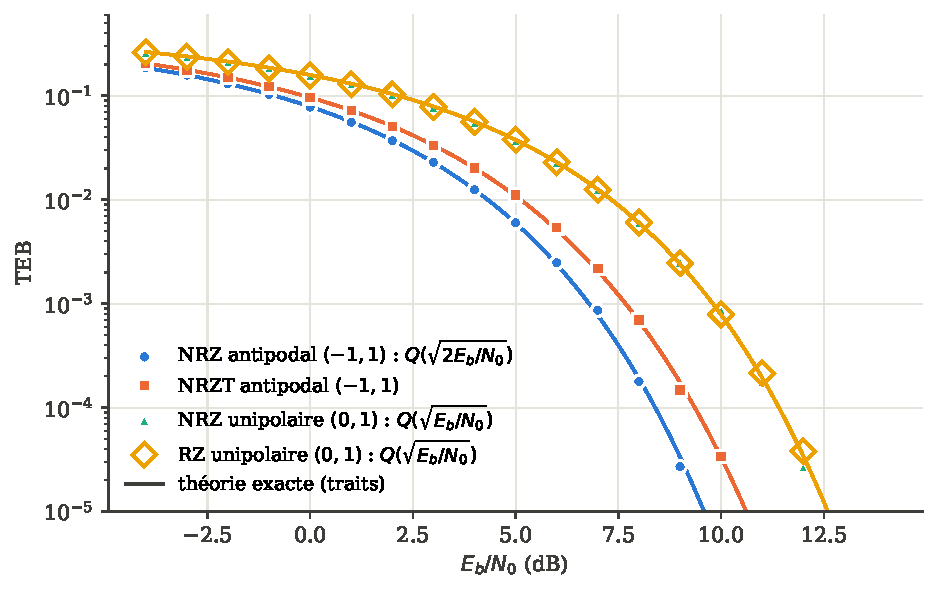
\includegraphics[width=0.85\linewidth]{../etape4/figures/fig_teb_filtre.pdf}
\caption{TEB du récepteur à filtre adapté (points) et théorie exacte (traits), canal gaussien sans écho.}\label{fig:tebfiltre}\end{figure}
Les points simulés se superposent à la théorie sur plus de quatre décades, jusqu'à $3\cdot10^{-5}$. L'écart médian entre simulation et théorie est de 0,8\,\%. L'écart relatif maximal (12\,\%) concerne des points à environ 170 erreurs, dont l'incertitude statistique relative est de l'ordre de $1/\sqrt{170} \approx 8\,\%$ : il représente 1,5 écart-type. Sur les 313 points simulés pour ce rapport, aucun ne s'écarte de la théorie de plus de 2,5 écarts-types (loi binomiale), ce qui est conforme à des fluctuations purement statistiques.
\begin{center}\begin{tabular}{lcccc}\toprule
& \multicolumn{2}{c}{4 dB} & \multicolumn{2}{c}{8 dB}\\
Configuration & simulé & théorie & simulé & théorie\\\midrule
NRZ antipodal $(-1,1)$ & $1{,}25\cdot10^{-2}$ & $1{,}25\cdot10^{-2}$ & $1{,}78\cdot10^{-4}$ & $1{,}91\cdot10^{-4}$\\
NRZT antipodal $(-1,1)$ & $2{,}01\cdot10^{-2}$ & $2{,}01\cdot10^{-2}$ & $7{,}0\cdot10^{-4}$ & $6{,}8\cdot10^{-4}$\\
NRZ unipolaire $(0,1)$ & $5{,}60\cdot10^{-2}$ & $5{,}65\cdot10^{-2}$ & $6{,}09\cdot10^{-3}$ & $6{,}00\cdot10^{-3}$\\
RZ unipolaire $(0,1)$ & $5{,}63\cdot10^{-2}$ & $5{,}65\cdot10^{-2}$ & $6{,}03\cdot10^{-3}$ & $6{,}00\cdot10^{-3}$\\\bottomrule
\end{tabular}\end{center}
Le NRZ unipolaire et le RZ unipolaire ont exactement la même courbe : avec le filtre adapté, seule compte l'énergie de la différence $s_1 - s_0$ rapportée à $E_b$, identique dans les deux cas (tableau de la section~\ref{sec:theorie}). Le NRZT perd environ 0,9~dB sur le NRZ : les rampes réduisent l'énergie utile de $g$ et le bit précédent crée une légère IES.

\subsection{Gain par rapport à l'étape 3}
\begin{figure}[htbp]\centering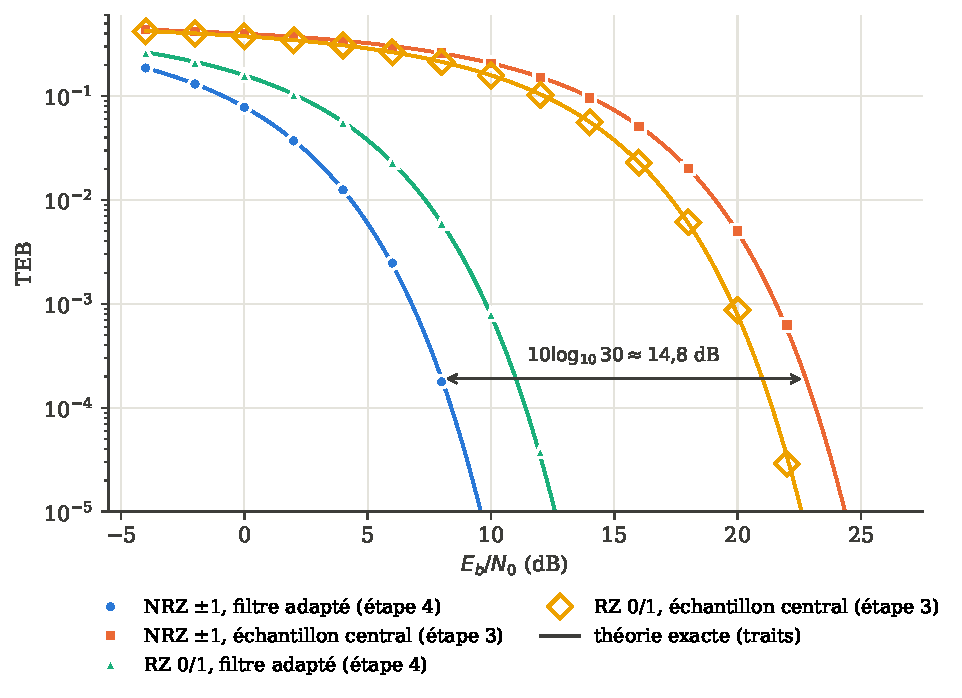
\includegraphics[width=0.85\linewidth]{../etape4/figures/fig_avant_apres.pdf}
\caption{Récepteur de l'étape 3 (échantillon central, recompilé depuis le commit \texttt{82e4660}) et récepteur à filtre adapté.}\label{fig:avantapres}\end{figure}
Le récepteur de l'étape 3 a été recompilé à partir du commit qui le contient encore et soumis aux mêmes balayages. Ses mesures suivent la théorie de la décision sur un échantillon ($0{,}258$ mesuré et théorique à 8~dB en NRZ). Le tableau donne le $\EbNo$ nécessaire pour atteindre un TEB de $10^{-3}$ (théorie exacte, confirmée par les points simulés) :
\begin{center}\begin{tabular}{lccc}\toprule
Forme & Étape 3 (échantillon central) & Étape 4 (filtre adapté) & Gain\\\midrule
NRZ antipodal $(-1,1)$ & 21,6 dB & 6,8 dB & \textbf{14,8 dB}\\
NRZT antipodal $(-1,1)$ & 21,1 dB & 7,7 dB & \textbf{13,4 dB}\\
RZ unipolaire $(0,1)$ & 19,8 dB & 9,8 dB & \textbf{10,0 dB}\\\bottomrule
\end{tabular}\end{center}
Le gain vaut $10\log_{10}M$, où $M$ est le nombre d'échantillons qui portent l'information : $M = N = 30$ en NRZ (14,8~dB), mais seulement $M = N/3 = 10$ en RZ (10~dB), dont seul le tiers central distingue un 1 d'un 0. En NRZT, les rampes rendent une partie des échantillons moins utiles, d'où un gain intermédiaire. Le RZ, qui paraissait meilleur que le NRZ à l'étape 3 (artefact de la décision ponctuelle, déjà expliqué dans le rapport précédent), retrouve sa place théorique : 3~dB derrière le NRZ antipodal.

\subsection{Trajets multiples sans bruit (étape 4a)}
\begin{figure}[htbp]\centering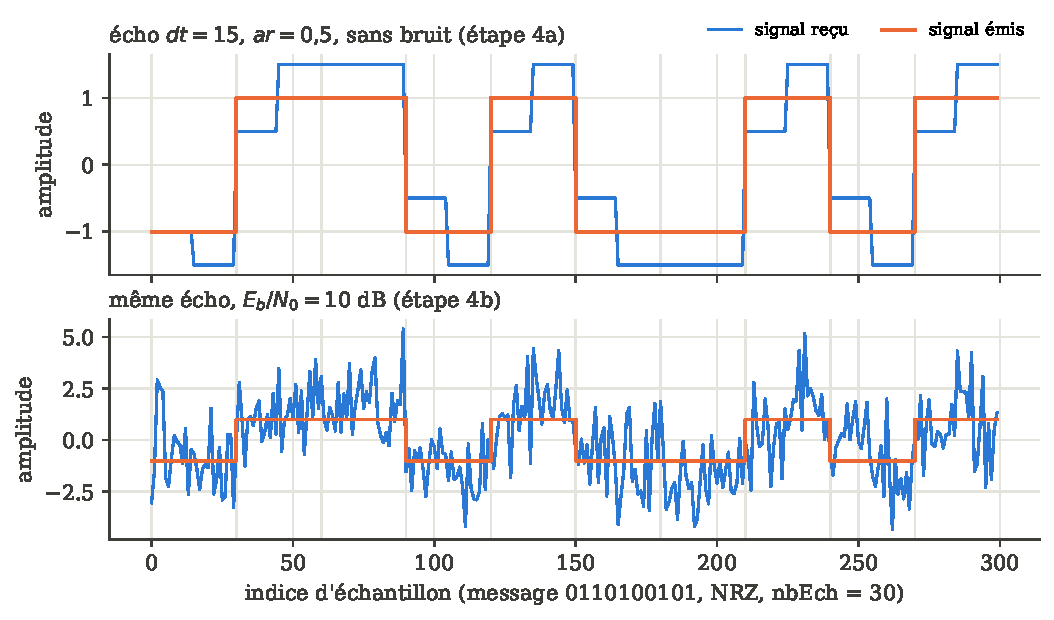
\includegraphics[width=0.9\linewidth]{../etape4/figures/fig_signal_echo.pdf}
\caption{Signal NRZ $(-1, 1)$ émis et reçu avec un écho $dt = 15$, $ar = 0{,}5$ (sortie des classes du simulateur via \texttt{ExportSignal}).}\label{fig:signal}\end{figure}
La figure~\ref{fig:signal} montre l'effet d'un écho retardé d'un demi-bit : la première moitié de chaque bit reçoit l'écho du bit précédent, la seconde celui du bit courant. Quand deux bits consécutifs sont égaux, l'écho renforce le signal ($1{,}5$) ; quand ils diffèrent, il l'atténue ($0{,}5$) sur la première moitié du bit.
\begin{figure}[htbp]\centering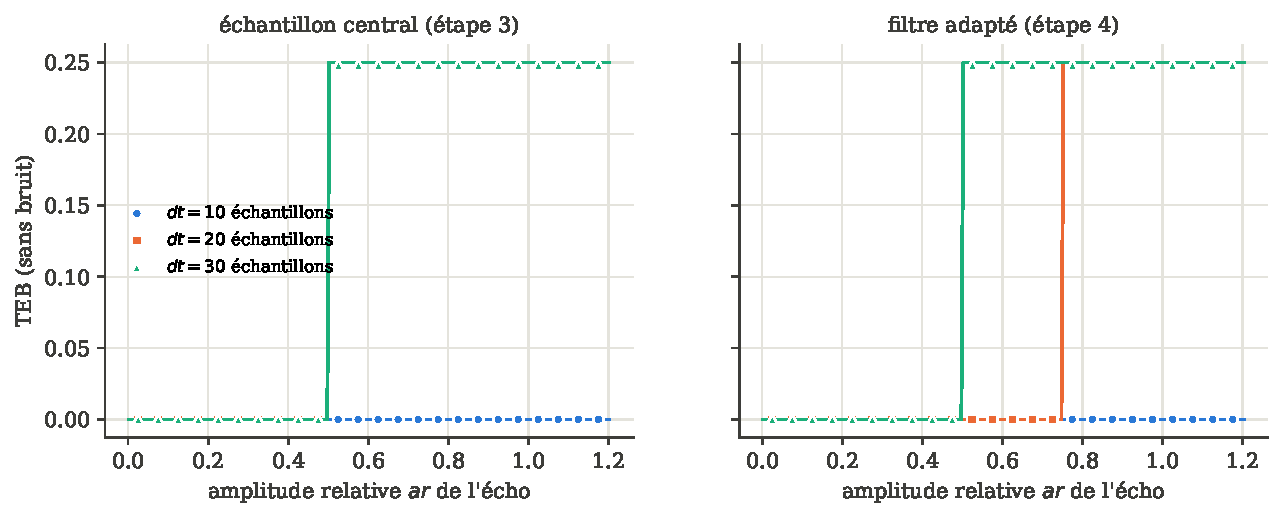
\includegraphics[width=\linewidth]{../etape4/figures/fig_trajets_alpha.pdf}
\caption{TEB sans bruit en fonction de l'amplitude de l'écho, NRZ unipolaire $(0,1)$ (amplitudes par défaut), un seul trajet indirect, 20\,000 bits par point. Pour $dt = 20$, la courbe de l'étape 3 est confondue avec celle de $dt = 30$.}\label{fig:alpha}\end{figure}
Sans bruit, le TEB est soit nul, soit égal à $1/4$ : toutes les erreurs viennent d'une même configuration, un bit 0 précédé d'un bit 1, dont l'écho fait franchir le seuil. Pour le NRZ unipolaire avec un écho $dt \le N$, la sortie du filtre adapté (ici $g = 1$, seuil $N/2$) se calcule directement. Les $dt$ premiers échantillons du bit courant $b$ reçoivent l'écho du bit précédent $p$, les autres celui du bit courant :
\[ y = \sum_{k<dt}(b + ar\,p) + \sum_{k\ge dt}(b + ar\,b) = N b + ar\,\big(dt\, p + (N - dt)\,b\big). \]
Pour $b = 0$ et $p = 1$, $y = ar\,dt$ dépasse le seuil $N/2$ dès que $ar > N/(2\,dt)$. Cette configuration a une probabilité $1/4$ :
\begin{center}\small\begin{tabularx}{\linewidth}{c>{\centering\arraybackslash}X>{\centering\arraybackslash}X>{\centering\arraybackslash}X}\toprule
$dt$ & seuil d'erreur, filtre adapté & mesuré (filtre adapté) & seuil d'erreur, étape 3\\\midrule
10 & $ar > 1{,}5$ & aucune erreur jusqu'à 1,175 (fin du balayage) & jamais (l'échantillon central voit l'écho du bit courant)\\
20 & $ar > 0{,}75$ & premières erreurs à 0,775 & $ar > 0{,}5$\\
30 & $ar > 0{,}5$ & premières erreurs à 0,525 & $ar > 0{,}5$\\\bottomrule
\end{tabularx}\end{center}
Le filtre adapté résiste mieux à un écho qui ne recouvre qu'une partie du bit ($dt = 20$) : il moyenne l'écho du bit précédent avec la partie saine du bit, alors que l'échantillon central tombe en plein dans l'écho. Pour un écho d'un bit entier ($dt = N$), les deux récepteurs sont équivalents. En NRZ antipodal $(-1, 1)$, le seuil est à 0 et, pour tout retard, $y \cdot \text{signe}(b) \ge N(1 - ar)$ : il faut $ar > 1$ pour une erreur, ce qui est physiquement exclu pour un trajet indirect ($ar < 1$) : c'est pourquoi le test JUnit des échos destructeurs utilise deux échos de $0{,}9$ qui s'additionnent.

\subsection{Trajets multiples et bruit (étape 4b)}
\begin{figure}[htbp]\centering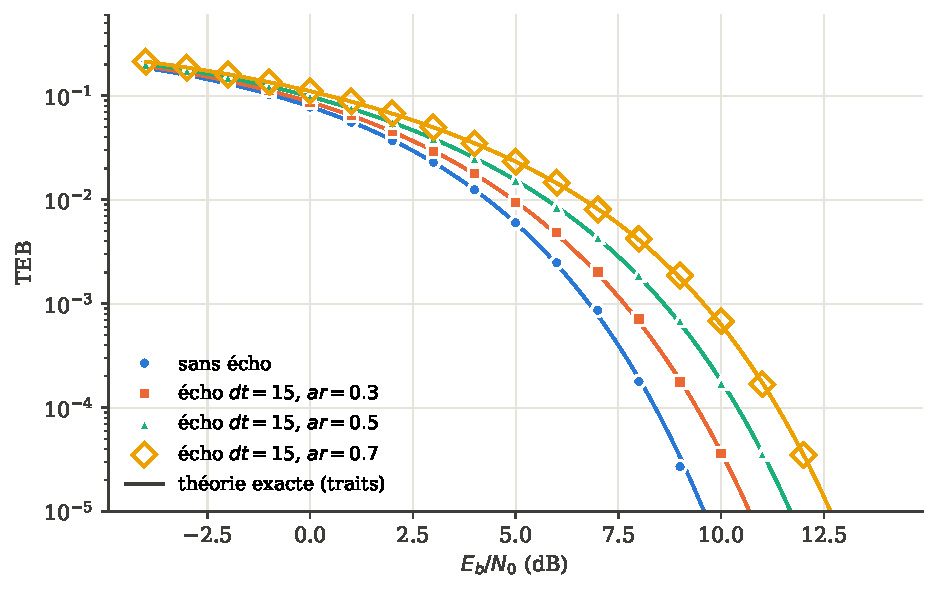
\includegraphics[width=0.85\linewidth]{../etape4/figures/fig_trajets_ebn0.pdf}
\caption{TEB en présence d'un écho $dt = 15$ (un demi-bit) et de bruit, NRZ antipodal $(-1, 1)$, filtre adapté.}\label{fig:ebn0}\end{figure}
Pour un écho d'un demi-bit en NRZ antipodal, le calcul de la section précédente donne deux cas équiprobables :
\begin{itemize}
  \item bits précédent et courant égaux : l'écho renforce tout le bit, la marge est multipliée par $(1 + ar)$ ;
  \item bits différents : l'écho du bit précédent et celui du bit courant se compensent exactement, la marge est celle d'un canal sans écho.
\end{itemize}
Mais la puissance reçue augmente, $P_s = \frac34(1 + ar)^2 + \frac14(1 - ar)^2$, et le bruit, réglé sur $E_b = P_s T$ mesuré après les échos (fiche de la séance 4), augmente dans la même proportion :
\[ \text{TEB} = \tfrac12\,Q\Big(\sqrt{2\EbNo / P_s}\Big) + \tfrac12\,Q\Big((1 + ar)\sqrt{2\EbNo / P_s}\Big). \]
\begin{center}\begin{tabular}{ccccc}\toprule
$ar$ & TEB à 8 dB (simulé) & TEB à 8 dB (théorie) & $\EbNo$ pour $10^{-3}$ & pénalité\\\midrule
0 & $1{,}78\cdot10^{-4}$ & $1{,}91\cdot10^{-4}$ & 6,8 dB & --\\
0,3 & $7{,}2\cdot10^{-4}$ & $6{,}7\cdot10^{-4}$ & 7,6 dB & 0,9 dB\\
0,5 & $1{,}88\cdot10^{-3}$ & $1{,}83\cdot10^{-3}$ & 8,6 dB & 1,8 dB\\
0,7 & $4{,}2\cdot10^{-3}$ & $4{,}1\cdot10^{-3}$ & 9,6 dB & 2,8 dB\\\bottomrule
\end{tabular}\end{center}
La pénalité reste inférieure à l'augmentation de puissance $10\log_{10}P_s$ (1,4 ; 2,4 ; 3,4~dB) : la moitié du temps, l'écho renforce la décision, ce qui compense en partie.

%======================================================================
\section{Confrontation aux prévisions}
\subsection{Ce qui est conforme}
\begin{itemize}
  \item \textbf{Filtre adapté} : le TEB rejoint la borne optimale ($1{,}25\cdot10^{-2}$ à 4~dB en NRZ antipodal, simulé et théorique) et le gain prévu de 14,8~dB est mesuré. Les 3~dB entre antipodal et unipolaire sont retrouvés.
  \item \textbf{Trajets multiples sans bruit} : le TEB est nul tant que l'écho ne fait pas franchir le seuil, puis vaut exactement la probabilité des suites défavorables ($1/4$). Les seuils d'apparition des erreurs mesurés correspondent au calcul ($ar > N/(2\,dt)$).
  \item \textbf{Trajets multiples et bruit} : le TEB augmente avec $ar$ à $\EbNo$ fixé, et la théorie exacte prédit chaque point.
\end{itemize}
\subsection{Ce qui diffère de l'intuition}
\begin{itemize}
  \item L'écho d'un bit entier est bien le plus gênant, mais seulement pour les amplitudes unipolaires, dont le seuil est à mi-hauteur : il provoque des erreurs dès $ar > 0{,}5$. En NRZ antipodal, un écho \emph{unique} d'amplitude $ar < 1$ ne crée jamais d'erreur sans bruit, quel que soit son retard ; il faut plusieurs échos qui s'additionnent.
  \item En 4b, une partie de la dégradation vient de la définition de $\EbNo$ : l'énergie de l'écho est comptée dans $E_b$ alors qu'elle n'est utile que la moitié du temps.
  \item Le RZ est robuste aux échos courts : son impulsion est concentrée dans le tiers central, et l'écho de l'impulsion précédente n'atteint le tiers central du bit courant que si $dt > 2N/3$. Vérifié par simulation (RZ $0/1$, 20\,000 bits, sans bruit) : aucune erreur pour $dt \in \{10, 15, 20\}$ jusqu'à $ar = 1{,}1$, alors qu'à $dt = 30$ le TEB vaut $0{,}25$ dès $ar = 0{,}7$.
\end{itemize}

%======================================================================
\section{Tests}
\subsection{Tests automatiques (\texttt{runTests})}
Le script couvre maintenant les étapes 1 à 4 dans des sections séparées ; chaque commentaire \texttt{\# Test n} correspond au numéro affiché. Six tests concernent l'étape 4 :
\begin{lstlisting}[language={}]
Test 15 : Trajets indirects (1 trajet, sans bruit) ... OK
Test 16 : Trajets indirects (1 trajet, bruité) ... OK
Test 17 : Trajets indirects (3 trajets, bruité) ... OK
Test 26 : Erreur (ti sans couple) ... OK
Test 27 : Erreur (ti sans valeur ar) ... OK
Test 28 : Erreur (ti plus de 5 couples) ... OK
------------------------------------------
  RÉSULTAT : 28/28 OK
\end{lstlisting}

\subsection{Tests unitaires JUnit}
La suite passe de 75 à \textbf{96 tests} (22 ajoutés, 1 supprimé), tous réussis. Tests ajoutés :
\begin{itemize}
  \item \textbf{canal à trajets multiples} (\cls{TransmetteurTest}, préfixe TATM) : écho appliqué seulement après son retard ; bruit reproductible avec une semence ; signal vide ; \emph{bruit identique à celui du canal gaussien sans trajet indirect} (vérifie le partage de la formule) ; rejet de tableaux incohérents, de plus de 5 trajets et d'un retard négatif ;
  \item \textbf{filtre adapté} (préfixe TAL) : en RZ, une forte perturbation hors du tiers central ne change pas la décision ; un échantillon central très faussé ne suffit plus à provoquer une erreur ; une séquence NRZT avec toutes les combinaisons de rampes est décodée sans erreur ;
  \item \textbf{simulateur} : \texttt{-ti} avec des échos destructeurs donne un TEB non nul ; \texttt{-ti} sans \texttt{-snrpb} n'ajoute pas de bruit ; un écho d'amplitude nulle donne exactement le même TEB que \texttt{-snrpb} seul ; \texttt{-ti} suivi d'autres options ; rejets des valeurs invalides ; \emph{TEB conforme à la théorie} : NRZ antipodal à 4~dB, $1{,}25\cdot10^{-2}$ à $\pm 12\,\%$ sur $10^5$ bits ;
  \item compléments de couverture ajoutés par L.~Nanda sur l'émetteur (rampes NRZT, forme inconnue, signal vide) et le canal gaussien.
\end{itemize}
Le dernier test simulateur répond à la limite relevée à l'étape 3 : les tests vérifiaient que le simulateur affichait un TEB, pas sa valeur.

\subsection{Limites identifiées}
\begin{itemize}
  \item \textbf{Semences liées.} Avec \texttt{-seed}, la source et le canal utilisent toujours la même semence, donc des suites pseudo-aléatoires liées. Utiliser \texttt{seed} et \texttt{seed + 1} garantirait leur indépendance. Les courbes restent conformes à la théorie, ce qui indique que l'effet est négligeable ici.
  \item \textbf{Mémoire.} \cls{Information} stocke des \texttt{Float} (objets) : une simulation de 200\,000 bits à 30 échantillons occupe environ 400~Mo. Les balayages sont donc découpés en tranches ; un stockage en \texttt{float[]} réduirait fortement l'empreinte.
  \item \textbf{Pas de compensation des échos.} Le filtre adapté est optimal contre le bruit, pas contre l'IES. Un égaliseur est nécessaire pour annuler les trajets multiples.
  \item Le rapport de l'étape 3 prévoyait une option pour conserver la décision sur l'échantillon central. La commande unique n'en prévoyant pas, la comparaison est faite en recompilant la version de l'étape 3 depuis git (script de courbes).
\end{itemize}

%======================================================================
\section{Conclusion}
Le canal à trajets multiples est intégré au simulateur avec l'option \texttt{-ti} de la commande unique, avec ou sans bruit. L'héritage de \cls{TransmetteurAnalogiqueBruite} garantit que le bruit est calculé de la même façon dans les deux canaux, ce qui a supprimé une erreur de facteur $N$ présente dans la première version.

Le récepteur à filtre adapté, annoncé comme prioritaire à la fin de l'étape 3, est en place. Une seule règle, la corrélation avec $g = s_1 - s_0$, sert aux trois formes d'onde. Le TEB mesuré atteint désormais la borne théorique, soit un gain de 14,8~dB en NRZ et 10~dB en RZ par rapport à l'étape 3. Toutes les mesures, avec ou sans échos, sont prédites par une théorie exacte de la chaîne, avec un écart médian inférieur à 1\,\%.

Le filtre adapté ne compense pas les échos : en présence de trajets multiples, le TEB reste dégradé (1,8~dB de pénalité pour un écho de 0,5 à un demi-bit) et, sans bruit, un écho fort impose un TEB de $1/4$ en unipolaire. Deux pistes pour la suite : un égaliseur, qui estime et soustrait l'écho des bits déjà décidés, et le codage de canal de l'étape 5, qui pourra maintenant être évalué sur un récepteur optimal.


\part{Étape 5 -- Codage de canal}
\section{Objectifs de l'étape 5}
L'étape 5 insère un \textbf{codage de canal} dans la chaîne, pour diminuer le TEB de la transmission bruitée (TP5). Le travail demandé comporte trois points :
\begin{enumerate}
  \item intégrer le codage : un codeur juste après la source, un décodeur juste avant la destination, activés par la nouvelle option \texttt{-codeur} (pas de codage par défaut) ;
  \item mesurer l'intérêt du procédé : quelle amélioration du TEB selon la forme d'onde et le rapport signal à bruit ;
  \item dire si le simulateur permet de mettre en évidence l'amélioration de la synchronisation émetteur/récepteur promise par le code.
\end{enumerate}
L'étape s'appuie sur le récepteur à filtre adapté de la partie~II : le gain du codage est mesuré sur une chaîne dont le TEB sans codage est déjà à la borne théorique.

\section{Chaîne implémentée}
\begin{figure}[htbp]\centering
\resizebox{\linewidth}{!}{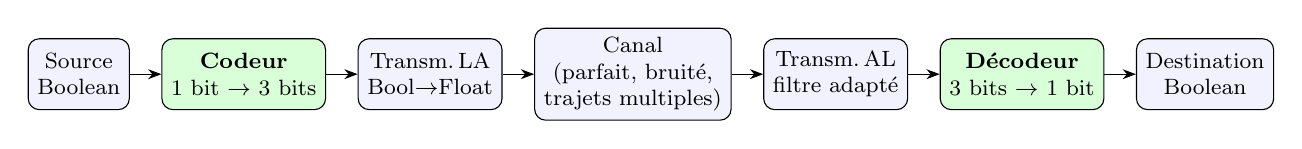
\begin{tikzpicture}[node distance=0.4cm,b/.style={draw,rounded corners,align=center,font=\footnotesize,minimum height=0.9cm,fill=blue!5},>=Stealth]
\node[b] (s) {Source\\Boolean};
\node[b,right=of s,fill=green!15] (co) {\textbf{Codeur}\\1 bit $\to$ 3 bits};
\node[b,right=of co] (e) {Transm.\,LA\\Bool$\to$Float};
\node[b,right=of e] (c) {Canal\\(parfait, bruité,\\trajets multiples)};
\node[b,right=of c] (r) {Transm.\,AL\\filtre adapté};
\node[b,right=of r,fill=green!15] (de) {\textbf{Décodeur}\\3 bits $\to$ 1 bit};
\node[b,right=of de] (d) {Destination\\Boolean};
\draw[->] (s)--(co); \draw[->] (co)--(e); \draw[->] (e)--(c); \draw[->] (c)--(r); \draw[->] (r)--(de); \draw[->] (de)--(d);
\end{tikzpicture}}
\caption{Chaîne de l'étape 5 avec l'option \texttt{-codeur}. En vert, les deux composants ajoutés. Le TEB est mesuré entre la source et la destination.}
\end{figure}
Sans \texttt{-codeur}, la chaîne est celle de l'étape 4. En simulation logique (aucune option analogique), le codeur et le décodeur entourent le transmetteur logique parfait.

\section{Récapitulatif des modifications depuis l'étape 4}
\begin{center}\small\begin{tabularx}{\linewidth}{>{\raggedright\arraybackslash}p{4.2cm}X}\toprule
Élément & Modification\\\midrule
\texttt{CodeurCanal} & Nouvelle classe (\texttt{Transmetteur<Boolean, Boolean>}) : chaque bit reçu est émis sur trois bits, $0 \to 010$ et $1 \to 101$.\\
\texttt{DecodeurCanal} & Nouvelle classe : chaque paquet de trois bits redonne un bit, par choix du mot de code le plus proche. Une erreur par paquet est corrigée.\\
\texttt{Simulateur} & Option \texttt{-codeur} ; la chaîne se branche sur deux extrémités logiques (source et destination, ou codeur et décodeur) ; sondes logiques du message émis et du message décodé avec \texttt{-s}. Option \texttt{-decalage d} (extension hors commande unique) pour désynchroniser le récepteur.\\
\texttt{TransmetteurAnalogique}\newline\texttt{Logique} & Décalage optionnel de la fenêtre de décision, pour simuler une désynchronisation (section~\ref{sec:desync}) ; 0 par défaut, résultats inchangés.\\
\texttt{VueDecalage} & Nouvelle classe : fenêtre interactive de désynchronisation (curseur, tracé des fenêtres de décision sur le signal, TEB recalculé), ouverte avec \texttt{-s -decalage}.\\
\texttt{InformationFlottante} & Nouvelle classe (sous-classe d'\texttt{Information<Float>}) : le signal analogique est rangé dans un tableau de \texttt{float} au lieu d'objets \texttt{Float}, pour réduire la mémoire (section~\ref{sec:perf}).\\
\texttt{TransmetteurLogique}\newline\texttt{Analogique},\newline\texttt{TransmetteurAnalogique}\newline\texttt{Bruite} & L'émetteur et le canal bruité (donc aussi le canal à trajets multiples) produisent une \texttt{InformationFlottante}. Leurs calculs sont inchangés.\\
Tests JUnit & 29 tests ajoutés : 125 tests, tous réussis.\\
\texttt{runTests} & Section « Étape 5 » : 6 exécutions nominales, dont un test de mémoire et deux tests de désynchronisation à TEB exact, et 3 tests d'erreur (37 tests).\\
\texttt{.gitignore} & Les fichiers générés (\texttt{bin/}, \texttt{docs/}) ne sont plus versionnés.\\
\texttt{genDeliverable}, \texttt{README} & Archive \texttt{etape5} ; description du contenu de l'archive et de l'option \texttt{-codeur}.\\
\texttt{rapport/etape5/} & Scripts \texttt{courbesCodage.py} (avec et sans codeur) et \texttt{courbesDecalage.py} (désynchronisation), avec théorie exacte ; outil \texttt{OutilsDecalage.java} (capture de la vue, paquets invalides).\\\bottomrule
\end{tabularx}\end{center}
Pour le codage de canal, aucune classe existante de la chaîne analogique n'a été modifiée. L'émetteur et le canal l'ont été ensuite, uniquement pour la façon de ranger le signal en mémoire : les TEB obtenus sont identiques au bit près.

\section{Prévisions avant simulation}
\subsection{Paramètres pertinents}
\begin{center}\begin{tabular}{lll}\toprule
Paramètre & Option & Rôle\\\midrule
Codage de canal & \texttt{-codeur} & active le codeur et le décodeur\\
Rapport $\EbNo$ (dB) & \texttt{-snrpb} & s'applique à chaque bit \emph{émis}, donc à chaque bit codé\\
Forme d'onde, amplitudes & \texttt{-form}, \texttt{-ampl} & fixent le TEB $p$ d'un bit codé\\
Trajets indirects & \texttt{-ti} & erreurs liées aux bits voisins\\\bottomrule
\end{tabular}\end{center}

\subsection{Résultats attendus}
\begin{itemize}
  \item \textbf{À \texttt{-snrpb} égal}, le TEB doit fortement diminuer. Si chaque bit codé est faux avec la probabilité $p$, indépendamment des autres, le décodeur se trompe quand au moins deux bits du paquet sont faux : $\text{TEB} = 3p^2 - 2p^3 \approx 3p^2$. L'amélioration doit donc être d'autant plus forte que $p$ est petit.
  \item \textbf{À énergie égale par bit d'information}, le résultat est moins évident : on émet trois bits pour un bit utile, donc trois fois plus d'énergie. Chaque bit codé ne dispose que du tiers de l'énergie, soit $10\log_{10}3 \approx 4{,}8$~dB de moins. Le codage n'est rentable que s'il regagne plus que ces 4,8~dB.
  \item \textbf{Forme d'onde} : le décodeur ne voit que des bits ; le gain exprimé en dB ne devrait presque pas dépendre de la forme d'onde.
  \item \textbf{Trajets multiples} : les erreurs dues aux échos ne sont pas indépendantes d'un bit à l'autre. Le code, conçu pour une erreur isolée par paquet, pourrait être moins efficace.
\end{itemize}

\section{Le codage retenu}
\subsection{Mots de code et décodage}
Le codeur associe à chaque bit un mot de trois bits : le bit, son inverse, puis le bit.
\begin{center}\begin{tabular}{cc}\toprule Bit & Mot émis\\\midrule 0 & 010\\ 1 & 101\\\bottomrule\end{tabular}
\qquad
\begin{tabular}{cccccccc}\toprule
000 & 001 & 010 & 011 & 100 & 101 & 110 & 111\\\midrule
0 & 1 & 0 & 0 & 1 & 1 & 0 & 1\\\bottomrule
\end{tabular}\end{center}
Les deux mots diffèrent sur leurs trois bits (distance de Hamming 3). Le décodeur choisit le mot le plus proche du paquet reçu (tableau de droite, celui du TP5) : un paquet qui contient une erreur est à distance 1 du bon mot et à distance 2 de l'autre, il est donc corrigé ; avec deux ou trois erreurs, le décodeur se trompe.

Ce code est un code à répétition dont le bit du milieu est inversé. Le mot le plus proche s'obtient donc par un vote majoritaire après avoir ré-inversé le bit du milieu, ce qui évite d'écrire les huit cas :
\begin{lstlisting}
// CodeurCanal.emettre()
for (boolean bit : informationRecue) {        // 0 -> 010, 1 -> 101
    informationEmise.add(bit);
    informationEmise.add(!bit);
    informationEmise.add(bit);
}

// DecodeurCanal.emettre()
for (int i = 0; i < nbPaquets; i++) {
    int debut = i * CodeurCanal.LONGUEUR_MOT;
    int votesPourUn = 0;
    if (informationRecue.iemeElement(debut))      votesPourUn++;
    if (!informationRecue.iemeElement(debut + 1)) votesPourUn++;   // bit du milieu inversé
    if (informationRecue.iemeElement(debut + 2))  votesPourUn++;
    informationEmise.add(votesPourUn >= 2);
}
\end{lstlisting}
Un test JUnit vérifie que ce vote reproduit les huit lignes de la table du TP5.

\subsection{Lecture en termes d'automate}
Le décodeur est un transducteur déterministe : il lit les bits trois par trois et, pour chacun des $2^3 = 8$ paquets possibles, il existe une et une seule sortie. Vu comme un automate, il part d'un état initial, compte les votes en lisant trois bits (au plus quatre états de comptage : 0, 1, 2 ou 3 votes pour « 1 »), émet un bit, puis revient à l'état initial. Le déterminisme a ici un intérêt pratique direct : le décodage ne demande ni retour en arrière ni mémoire au-delà du paquet en cours, et son coût est proportionnel à la longueur du message.

\subsection{Intégration dans le simulateur}
Le codeur et le décodeur sont des \texttt{Transmetteur<Boolean, Boolean>}, comme le transmetteur parfait de l'étape 1. Le simulateur définit deux « extrémités logiques », entre lesquelles il branche la chaîne logique ou analogique sans autre changement :
\begin{lstlisting}
SourceInterface<Boolean> entree = source;
DestinationInterface<Boolean> sortie = destination;
if (codageCanal) {                       // option -codeur
    CodeurCanal codeur = new CodeurCanal();
    DecodeurCanal decodeur = new DecodeurCanal();
    source.connecter(codeur);
    decodeur.connecter(destination);
    entree = codeur;
    sortie = decodeur;
}
// ... entree.connecter(emetteur); ... recepteur.connecter(sortie);
\end{lstlisting}
L'option \texttt{-codeur} ne prend pas de paramètre, conformément à la commande unique. Elle se combine avec toutes les autres options (\texttt{-form}, \texttt{-snrpb}, \texttt{-ti}, \texttt{-s}).

\subsection{TEB théorique après décodage}\label{sec:theoriecodage}
Le bruit est indépendant d'un bit codé à l'autre. Pour une suite de bits donnée, les erreurs sur les trois bits d'un paquet sont donc indépendantes, de probabilités $p_1$, $p_2$, $p_3$, et
\[ \text{TEB} = p_1p_2 + p_1p_3 + p_2p_3 - 2\,p_1p_2p_3 \qquad (= 3p^2 - 2p^3 \text{ si } p_1 = p_2 = p_3 = p). \]
En NRZ et en RZ sans écho, $p$ est le TEB sans codage de la partie~II. En NRZT et avec des échos, les $p_i$ dépendent des bits voisins. Le script \texttt{courbesCodage.py} énumère alors les suites de trois bits d'information, les code, reconstruit la fenêtre reçue de chaque bit du dernier paquet et moyenne la formule ci-dessus ; la puissance $P_s$ qui règle le bruit est celle du signal \emph{codé}.

\section{Résultats}
Les courbes sont produites par \texttt{rapport/etape5/courbesCodage.py}, avec $N = 30$. Les points sont simulés par notre simulateur (jusqu'à 600\,000 bits d'information par point avec codeur, $10^6$ sans) ; les traits sont la théorie exacte. Sur les 117 points simulés, aucun ne s'écarte de la théorie de plus de 2,5 écarts-types statistiques.

\subsection{Amélioration du TEB à \texttt{-snrpb} égal}
\begin{figure}[htbp]\centering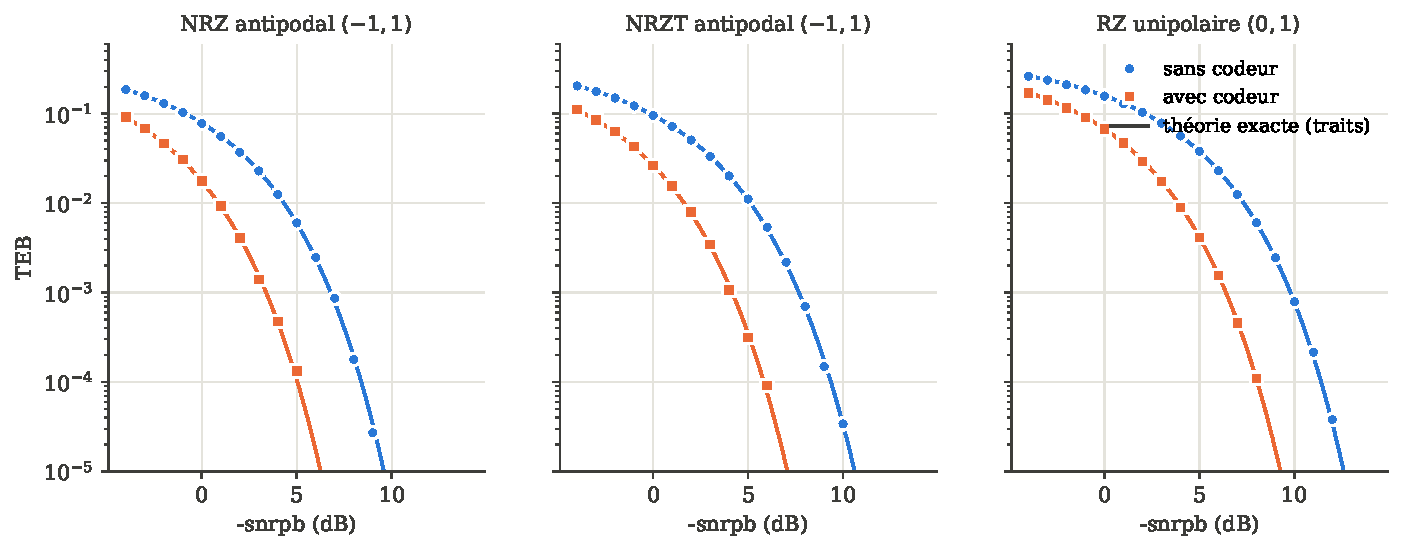
\includegraphics[width=\linewidth]{figures/fig_codage_formes.pdf}
\caption{TEB avec et sans codeur pour les trois formes d'onde, en fonction de \texttt{-snrpb} (rapport $\EbNo$ de chaque bit émis).}\label{fig:codageformes}\end{figure}
\begin{center}\begin{tabular}{lcccc}\toprule
& \multicolumn{2}{c}{\texttt{-snrpb 2}} & \multicolumn{2}{c}{\texttt{-snrpb 4}}\\
Configuration (simulé / théorie) & sans codeur & avec codeur & sans codeur & avec codeur\\\midrule
NRZ $(-1,1)$ & $3{,}71$ / $3{,}75\cdot10^{-2}$ & $4{,}05$ / $4{,}11\cdot10^{-3}$ & $1{,}25$ / $1{,}25\cdot10^{-2}$ & $4{,}75$ / $4{,}65\cdot10^{-4}$\\
NRZT $(-1,1)$ & $5{,}07$ / $5{,}10\cdot10^{-2}$ & $7{,}98$ / $7{,}66\cdot10^{-3}$ & $2{,}01$ / $2{,}01\cdot10^{-2}$ & $1{,}07$ / $1{,}21\cdot10^{-3}$\\
RZ $(0,1)$ & $1{,}03$ / $1{,}04\cdot10^{-1}$ & $2{,}94$ / $3{,}02\cdot10^{-2}$ & $5{,}63$ / $5{,}65\cdot10^{-2}$ & $8{,}95$ / $9{,}21\cdot10^{-3}$\\\bottomrule
\end{tabular}\end{center}
À \texttt{-snrpb} égal, le codage améliore nettement le TEB, et d'autant plus que le bruit est faible : le TEB est divisé par 9 à 2~dB et par 27 à 4~dB en NRZ antipodal, conformément à $3p^2$. Pour atteindre un TEB de $10^{-3}$ :
\begin{center}\begin{tabular}{lccc}\toprule
Forme & \texttt{-snrpb} sans codeur & \texttt{-snrpb} avec codeur & Gain\\\midrule
NRZ antipodal $(-1,1)$ & 6,8 dB & 3,4 dB & 3,4 dB\\
NRZT antipodal $(-1,1)$ & 7,7 dB & 4,2 dB & 3,5 dB\\
RZ unipolaire $(0,1)$ & 9,8 dB & 6,4 dB & 3,4 dB\\\bottomrule
\end{tabular}\end{center}
Le gain est pratiquement le même pour les trois formes d'onde : le décodeur ne traite que des bits, la forme d'onde ne fait que fixer $p$. Le léger écart du NRZT vient de la statistique du signal codé, qui change de valeur plus souvent (voir section~\ref{sec:codagetrajets}) : les rampes sont plus fréquentes et la puissance $P_s$ un peu plus faible.

\subsection{Comparaison à énergie égale par bit d'information}
\begin{figure}[htbp]\centering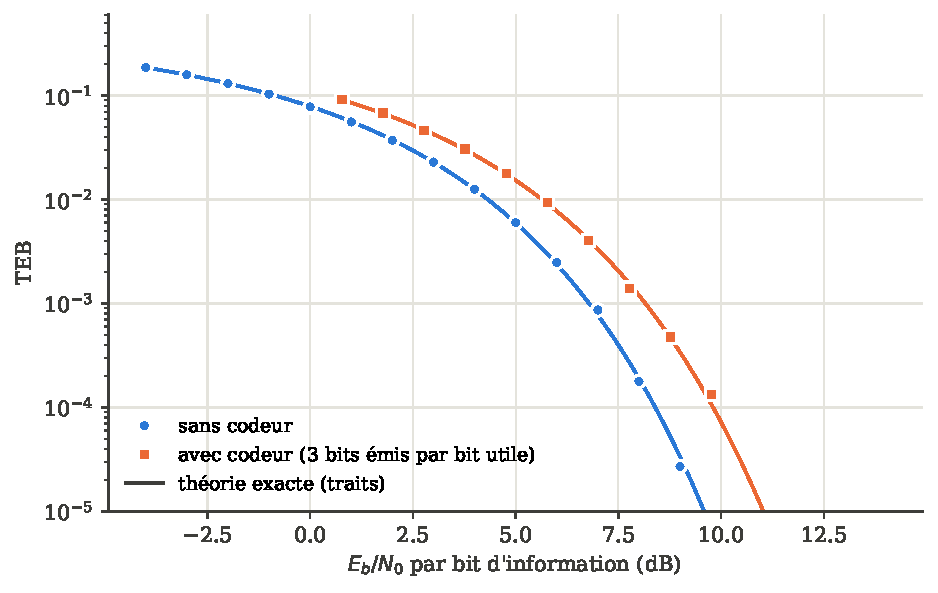
\includegraphics[width=0.85\linewidth]{figures/fig_codage_equitable.pdf}
\caption{NRZ antipodal : TEB en fonction de $\EbNo$ par bit d'information. Avec le codeur, l'énergie d'un bit utile est celle de ses trois bits codés ; la courbe est celle de la figure~\ref{fig:codageformes}, décalée de $10\log_{10}3 = 4{,}8$~dB.}\label{fig:equitable}\end{figure}
La comparaison précédente avantage le codage : avec \texttt{-codeur}, le simulateur émet trois bits par bit utile, chacun avec la même énergie. La transmission consomme donc trois fois plus d'énergie et, à débit d'émission constant, dure trois fois plus longtemps. Si l'on raisonne à énergie égale par bit d'information, la courbe codée se décale de 4,8~dB vers la droite (figure~\ref{fig:equitable}) et passe \emph{au-dessus} de la courbe sans codage :
\begin{center}\begin{tabular}{lccc}\toprule
$\EbNo$ par bit utile pour $10^{-3}$ & sans codeur & avec codeur & bilan\\\midrule
NRZ antipodal $(-1,1)$ & 6,8 dB & 8,2 dB & perte de 1,4 dB\\
NRZT antipodal $(-1,1)$ & 7,7 dB & 8,9 dB & perte de 1,3 dB\\
RZ unipolaire $(0,1)$ & 9,8 dB & 11,2 dB & perte de 1,4 dB\\\bottomrule
\end{tabular}\end{center}
Le code regagne 3,4~dB par la correction d'erreur, mais en dépense 4,8 par sa redondance. Ce résultat est connu : le gain de codage asymptotique d'un code de rendement $R$ qui corrige $t$ erreurs, décodé par décisions fermes, vaut $10\log_{10}\big(R\,(t+1)\big)$~[2], soit ici $10\log_{10}(2/3) = -1{,}8$~dB. Nos mesures ($-1{,}3$ à $-1{,}4$~dB entre $10^{-2}$ et $10^{-5}$) tendent vers cette valeur. Un décodage souple, qui additionnerait les trois sorties du filtre adapté avant de décider, ramènerait aux performances sans codage : un code à répétition n'apporte pas de gain de codage, il échange du débit contre de la fiabilité.

\textbf{Réponse à la question 2 du TP5.} Le codage améliore le TEB à puissance d'émission et rapport signal à bruit par bit émis constants (gain de 3,4~dB, quelle que soit la forme d'onde), au prix d'un débit utile divisé par trois. Il ne constitue pas une amélioration à énergie constante par bit d'information. Son intérêt pratique est donc de fiabiliser une liaison dont on ne peut pas augmenter la puissance, quand on accepte de réduire le débit.

\subsection{Codage et trajets multiples}\label{sec:codagetrajets}
\begin{figure}[htbp]\centering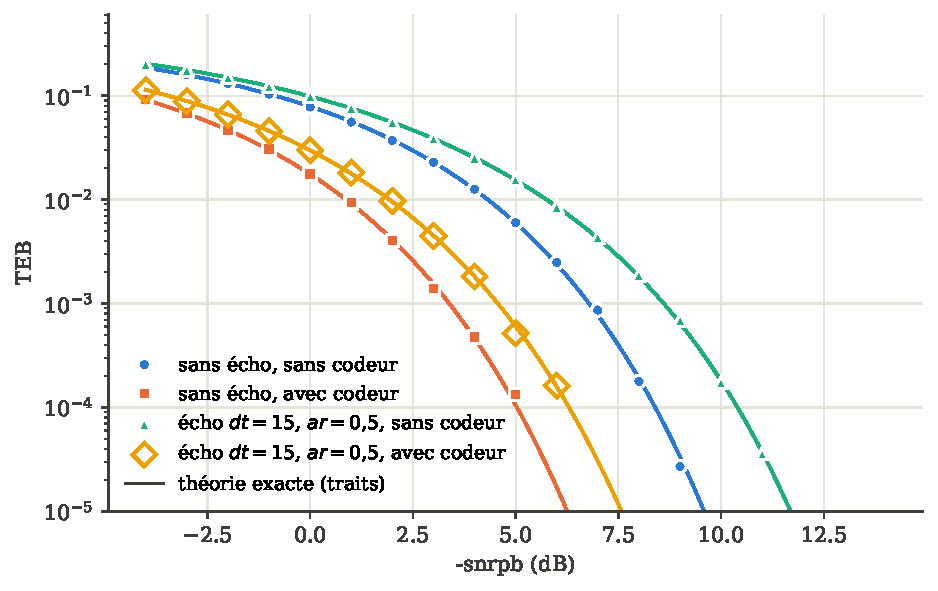
\includegraphics[width=0.85\linewidth]{figures/fig_codage_trajets.pdf}
\caption{NRZ antipodal $(-1,1)$, avec et sans écho ($dt = 15$, $ar = 0{,}5$), avec et sans codeur.}\label{fig:codagetrajets}\end{figure}
\textbf{Avec bruit (étape 4b).} Le codage reste efficace en présence d'un écho, et la pénalité due à l'écho est même plus faible avec le codeur :
\begin{center}\begin{tabular}{lccc}\toprule
\texttt{-snrpb} pour $10^{-3}$ & sans écho & écho $dt = 15$, $ar = 0{,}5$ & pénalité de l'écho\\\midrule
sans codeur & 6,8 dB & 8,6 dB & 1,8 dB\\
avec codeur & 3,4 dB & 4,6 dB & 1,2 dB\\\bottomrule
\end{tabular}\end{center}
L'explication tient à la forme du signal codé. Sans codage, deux bits consécutifs diffèrent une fois sur deux. Avec le code, les trois bits d'un mot alternent toujours, et seul le passage d'un mot au suivant peut conserver la valeur : deux bits consécutifs diffèrent 5 fois sur 6. Or, pour un écho d'un demi-bit, la partie~II a montré que l'écho n'aide la décision que si les bits sont égaux, et que le bruit est réglé sur la puissance reçue $P_s$. Avec le signal codé, $P_s = \frac16(1+ar)^2 + \frac56\cdot\frac12\big[(1-ar)^2 + (1+ar)^2\big] = 1{,}42$ pour $ar = 0{,}5$, contre $1{,}75$ sans codage : le bruit ajouté pour un même \texttt{-snrpb} est plus faible.

\textbf{Sans bruit (étape 4a).} En NRZ unipolaire $(0,1)$, où un écho fort fait franchir le seuil (partie~II), le codage n'apporte rien :
\begin{center}\begin{tabular}{ccccc}\toprule
$dt$ & $ar$ & sans codeur (simulé) & avec codeur (simulé) & théorie (les deux)\\\midrule
30 & 0,4 & 0 & 0 & 0\\
30 & 0,6 & 0,248 & 0,248 & 0,25\\
20 & 0,6 & 0 & 0 & 0\\
20 & 0,9 & 0,248 & 0,248 & 0,25\\
10 & 0,9 & 0 & 0 & 0\\\bottomrule
\end{tabular}\end{center}
Sans bruit, un bit 0 est faux chaque fois qu'il suit un bit 1 dont l'écho dépasse le seuil. Dans le mot $010$ qui suit un mot $101$, le premier et le troisième bit sont deux 0 précédés d'un 1 : le paquet contient deux erreurs, que le décodeur ne peut pas corriger. Ce cas se produit quand un bit d'information 0 suit un bit 1, soit une fois sur quatre : le TEB vaut $1/4$, comme sans codage. Le code corrige des erreurs isolées et aléatoires ; il est sans effet contre des erreurs systématiques, liées au signal lui-même. Contre les échos, il faut un égaliseur.

\subsection{Synchronisation émetteur/récepteur}
Dans le simulateur, le récepteur connaît le début de chaque bit : la synchronisation est parfaite par construction. La question 3 du TP5, qui porte sur l'amélioration de la synchronisation, demande donc de pouvoir simuler une désynchronisation. Elle fait l'objet de la section suivante.

\section{Désynchronisation du récepteur (question 3 du TP5)}\label{sec:desync}
La question 3 du TP5 demande si le simulateur permet de mettre en évidence l'amélioration de la synchronisation émetteur/récepteur promise par le code. Pour y répondre, nous avons rendu la fenêtre de décision du récepteur réglable : on peut ainsi simuler une désynchronisation et observer son effet sur les signaux et sur le TEB.

\subsection{Modèle et réalisation}
Par défaut, l'émetteur et le récepteur partagent la même base de temps : le bit $i$ occupe les échantillons $iN$ à $(i+1)N - 1$, et le récepteur intègre cette fenêtre. La synchronisation est parfaite. Nous modélisons une erreur de synchronisation constante par un décalage $d$ de la fenêtre de décision :
\[ \text{fenêtre du bit } i = \big[\, iN + d,\ iN + d + N \,\big[, \qquad |d| < N, \]
$d > 0$ correspondant à un récepteur en retard sur l'émetteur et $d < 0$ à un récepteur en avance. La fenêtre mord donc sur le bit suivant ou sur le bit précédent. Avant le début et après la fin du signal, rien n'est reçu (échantillons nuls).
\begin{lstlisting}
// TransmetteurAnalogiqueLogique.emettre()
// filtre adapté sur la fenêtre décalée
for (int i = 0; i < nbBits; i++) {
    int debutFenetre = i * nbEch + decalage;
    double y = 0.0;
    for (int k = 0; k < nbEch; k++) {
        y += echantillonRecu(debutFenetre + k) * filtre[k];   // 0 hors du signal
    }
    informationEmise.add(y > seuil);
}
\end{lstlisting}
\begin{itemize}
  \item \textbf{Option \texttt{-decalage d}} : le simulateur crée un récepteur décalé de $d$ échantillons, et le TEB affiché tient compte de la désynchronisation. Cette option n'existe pas dans la commande unique : c'est une extension, sans effet quand elle est absente. La borne $|d| < N$ est vérifiée une fois toutes les options lues, puisque \texttt{-nbEch} peut venir après.
  \item \textbf{Fenêtre interactive} : avec \texttt{-s -decalage d}, la fenêtre \cls{VueDecalage} s'ouvre après la simulation. Un curseur, ou la molette, fait varier $d$ de $-(N-1)$ à $N-1$ ; le signal reçu est de nouveau décidé (et décodé avec \texttt{-codeur}) à chaque mouvement, le tracé montre les fenêtres de décision sur le signal et le TEB du message complet est recalculé (figure~\ref{fig:vuedecalage}).
  \item Sans décalage, les résultats sont identiques au bit près à ceux de la version précédente.
\end{itemize}

\subsection{Effet sur les signaux}
\begin{figure}[htbp]\centering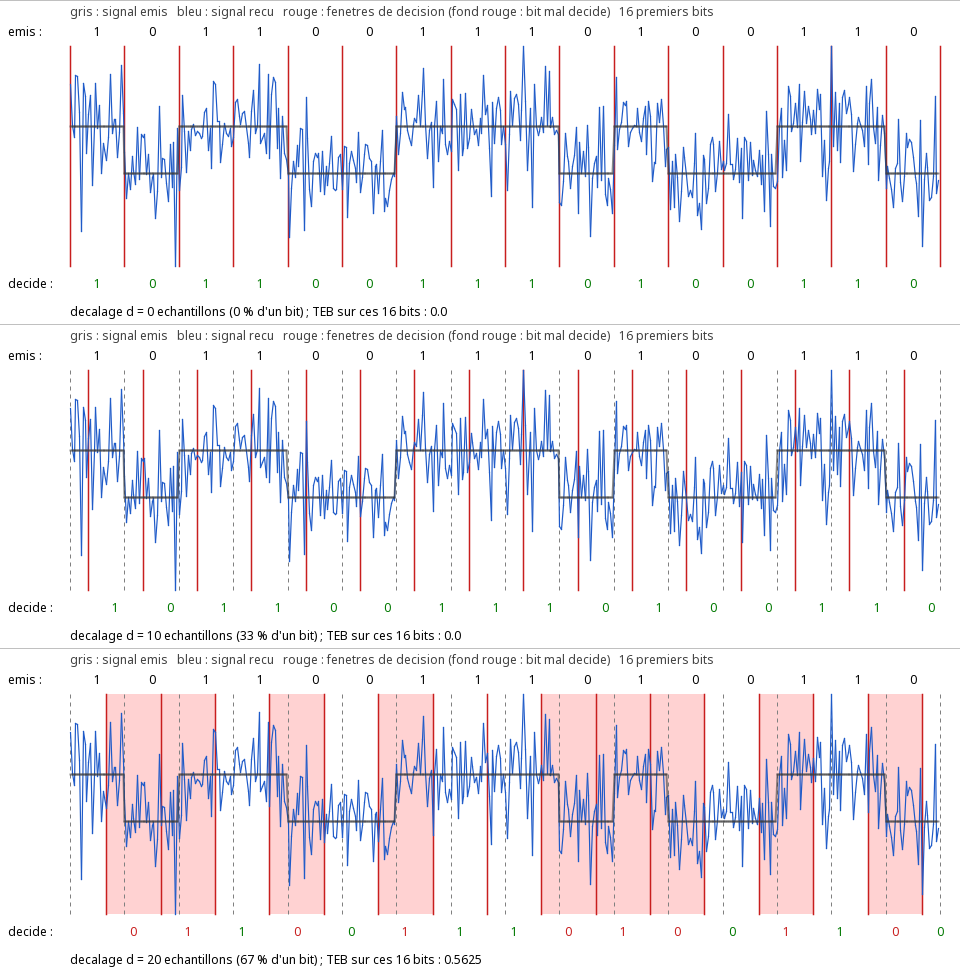
\includegraphics[width=\linewidth]{figures/fig_decalage_vue.png}
\caption{Tracé de la fenêtre interactive (NRZ antipodal, $\EbNo = 10$~dB, 16 premiers bits) pour $d = 0$, $10$ et $20$ échantillons. Gris : signal émis ; bleu : signal reçu ; pointillés : limites des bits ; traits rouges : fenêtres de décision ; fond rouge : bit mal décidé.}\label{fig:vuedecalage}\end{figure}
Avec $d = 10$ (un tiers de bit), chaque fenêtre contient deux tiers du bit courant et un tiers du bit suivant : la décision reste juste. Avec $d = 20$, chaque fenêtre contient davantage du bit suivant que du bit courant : le récepteur décide le bit suivant, et toutes les fenêtres où le bit change sont fausses.

\subsection{Effet sur le TEB sans bruit}
\begin{figure}[htbp]\centering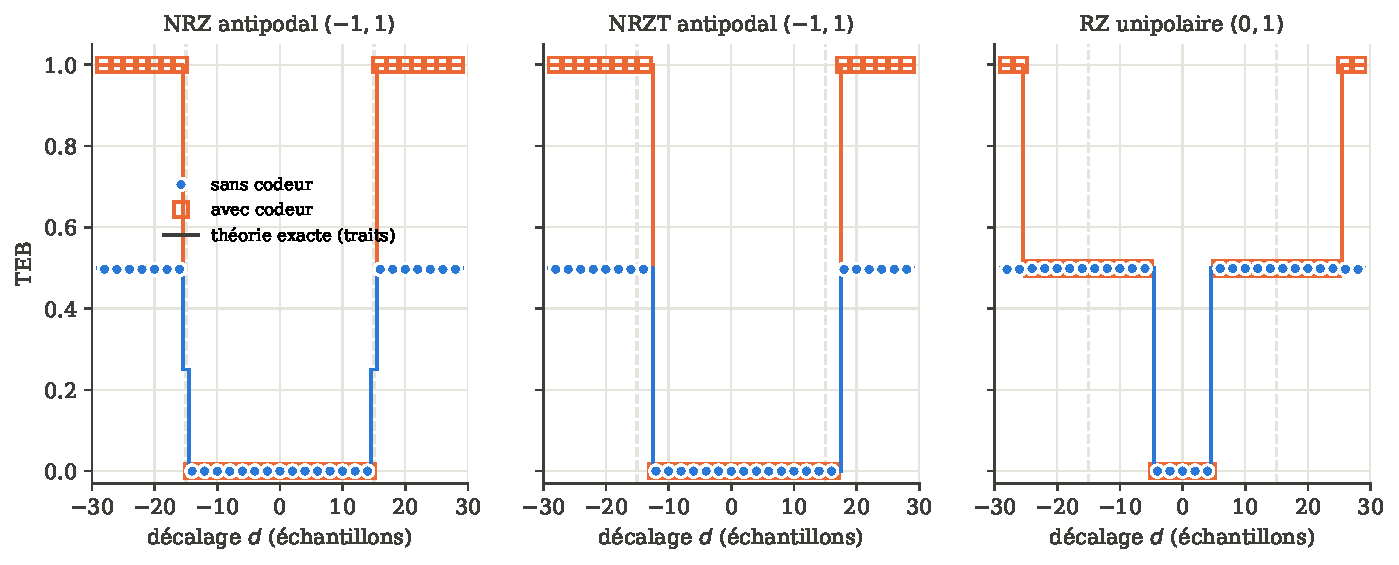
\includegraphics[width=\linewidth]{figures/fig_decalage_sans_bruit.pdf}
\caption{TEB sans bruit en fonction du décalage $d$ ($N = 30$), avec et sans codeur. Points : simulations (20\,000 bits, un point sur deux tracé) ; traits : théorie exacte. Pointillés : $|d| = N/2$.}\label{fig:decalagesansbruit}\end{figure}
Sans bruit, le TEB est nul tant que la fenêtre contient davantage du bit courant que de son voisin, puis saute brusquement :
\begin{center}\begin{tabular}{lccc}\toprule
Forme & décalages sans erreur & TEB au-delà, sans codeur & TEB au-delà, avec codeur\\\midrule
NRZ antipodal $(-1,1)$ & $-14 \le d \le 14$ & 0,5 & 1\\
NRZT antipodal $(-1,1)$ & $-12 \le d \le 17$ & 0,5 & 1\\
RZ unipolaire $(0,1)$ & $-4 \le d \le 4$ & 0,5 & 0,5, puis 1 si $|d| \ge 26$\\\bottomrule
\end{tabular}\end{center}
\begin{itemize}
  \item \textbf{NRZ} : la sortie du filtre vaut $2\big[(N - |d|)\,s_i + |d|\,s_{\text{voisin}}\big]$. Tant que $|d| < N/2$, le bit courant l'emporte. Au-delà, le récepteur décide la valeur du voisin, et se trompe chaque fois que les deux bits diffèrent, soit une fois sur deux.
  \item \textbf{NRZT} : la tolérance est dissymétrique. Un récepteur en retard ($d > 0$) saute la rampe du début du bit, qui dépend du bit précédent, et n'atteint que la rampe du bit suivant, qui part du niveau du bit courant : il tolère jusqu'à 17 échantillons. En avance, il intègre la fin du bit précédent et ne tolère que 12 échantillons.
  \item \textbf{RZ} : l'impulsion n'occupe que le tiers central du bit. Dès que la fenêtre se décale de la moitié de cette impulsion ou plus ($N/6 = 5$ échantillons), elle ne voit plus assez d'impulsion pour décider un 1 : tous les bits 1 sont perdus. C'est la forme d'onde la plus sensible à la désynchronisation. Pour $|d| \ge 26$, la fenêtre voit au contraire plus de la moitié de l'impulsion du bit \emph{voisin}, et décide ce bit.
  \item \textbf{Avec le codeur}, la tolérance est la même, mais au-delà le TEB vaut 1 en NRZ et NRZT : \emph{tout le message est inversé}. Le récepteur lit, pour le paquet $(b, \bar b, b)$, les bits $(\bar b, b, b')$ ; après ré-inversion du bit du milieu, le vote majoritaire donne toujours $\bar b$. En RZ, pour $5 \le |d| \le 25$, toutes les décisions valent 0 et le décodeur rend 0 pour chaque paquet : le TEB reste de 0,5 ; pour $|d| \ge 26$, le récepteur lit le bit voisin et le message est de nouveau inversé.
\end{itemize}

\subsection{Effet sur le TEB avec bruit}
\begin{figure}[htbp]\centering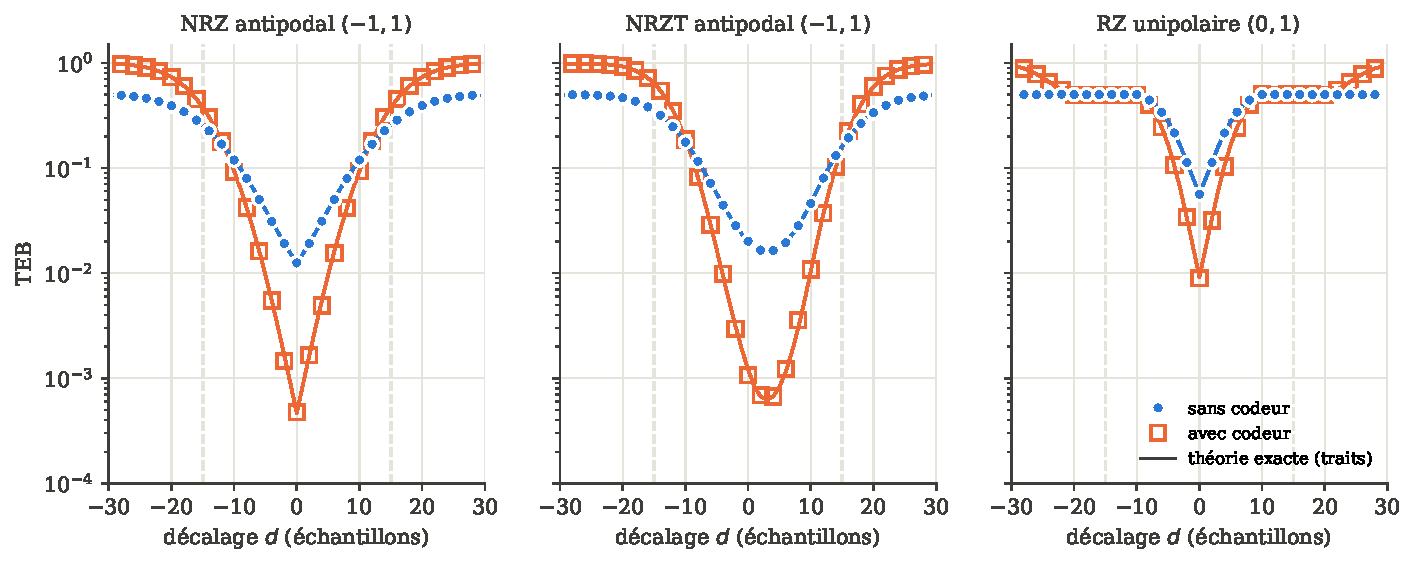
\includegraphics[width=\linewidth]{figures/fig_decalage_bruit.pdf}
\caption{TEB en fonction du décalage $d$ à $\EbNo = 4$~dB, avec et sans codeur. Points : simulations ; traits : théorie exacte.}\label{fig:decalagebruit}\end{figure}
Valeurs mesurées et théoriques en NRZ antipodal (TEB) :
\begin{center}\footnotesize\begin{tabular}{lccccccc}\toprule
$d$ (échantillons) & $-10$ & $-4$ & $0$ & $4$ & $10$ & $14$ & $20$\\\midrule
sans codeur, simulé & 0,119 & 0,031 & 0,0125 & 0,0313 & 0,119 & 0,227 & 0,392\\
sans codeur, théorie & 0,12 & 0,0313 & 0,0125 & 0,0313 & 0,12 & 0,227 & 0,393\\\midrule
avec codeur, simulé & 0,0921 & 0,00548 & 0,000475 & 0,00493 & 0,0934 & 0,306 & 0,735\\
avec codeur, théorie & 0,0939 & 0,00549 & 0,000465 & 0,00549 & 0,0939 & 0,306 & 0,735\\
\bottomrule\end{tabular}\end{center}
\begin{itemize}
  \item Avec du bruit, il n'y a plus de tolérance : le TEB augmente dès le premier échantillon de décalage, car la partie du voisin réduit la marge de décision. En NRZ, un décalage d'un sixième de bit ($d = 5$) triple déjà le TEB.
  \item Le codeur reste utile pour les petits décalages, mais devient nuisible au-delà d'environ $|d| = 12$ en NRZ : son TEB tend vers 1 alors que celui sans codeur tend vers 0,5. En NRZT, le croisement a lieu à $d = 16$ en retard mais dès $d = -10$ en avance ; en RZ, les deux TEB valent 0,5 dès $|d| \ge 10$.
  \item L'effet est rapide : en NRZ, une erreur de synchronisation d'un tiers de bit multiplie le TEB par 10 sans codeur et par 200 avec codeur.
\end{itemize}

\subsection{Le code permet de détecter une désynchronisation}
Le code ne protège donc pas contre une erreur de synchronisation. Sa structure permet en revanche de la détecter. Quand le récepteur est synchronisé, les paquets reçus sont des mots de code ($010$ ou $101$), sauf erreur due au bruit. Quand il est décalé de plus d'un demi-bit, il lit $(\bar b, b, b')$, qui n'est un mot de code que si $b' \ne b$ : un paquet sur deux n'en est plus un.
\begin{center}\footnotesize\begin{tabular}{lcccccc}\toprule
NRZ antipodal, avec codeur, $d$ & $0$ & $5$ & $10$ & $14$ & $16$ & $20$\\\midrule
sans bruit : paquets invalides & 0,0~\% & 0,0~\% & 0,0~\% & 0,0~\% & 50,3~\% & 50,3~\%\\
sans bruit : TEB & 0 & 0 & 0 & 0 & 1 & 1\\\midrule
4 dB : paquets invalides & 3,8~\% & 16,5~\% & 46,8~\% & 71,2~\% & 77,1~\% & 73,8~\%\\
4 dB : TEB & 0,000333 & 0,00973 & 0,0947 & 0,307 & 0,451 & 0,733\\
\bottomrule\end{tabular}\end{center}
Un récepteur qui surveille la proportion de paquets invalides peut donc repérer une désynchronisation, avant même que le TEB ne s'effondre, et se recaler (par exemple en essayant les trois positions possibles du début des paquets et en gardant celle qui donne le moins de paquets invalides). C'est un premier apport concret du code à la synchronisation.

\subsection{Réponse à la question 3}
\textbf{En partie.} Le simulateur permet désormais de :
\begin{itemize}
  \item simuler une désynchronisation constante et observer son effet sur les signaux (fenêtre interactive) et sur le TEB (option \texttt{-decalage}) ;
  \item vérifier que le code ne protège pas contre une erreur de synchronisation : il la rend même catastrophique au-delà d'un demi-bit (message inversé) ;
  \item montrer que le code permet de la détecter (paquets invalides), et vérifier la propriété annoncée par le TP : jamais plus de deux bits consécutifs identiques dans le signal codé (test JUnit).
\end{itemize}
L'amélioration promise par le TP concerne cependant la récupération du rythme : un récepteur réel recale en permanence son horloge sur les transitions du signal reçu, et une longue suite de bits identiques, sans transition, le laisse dériver. Notre modèle utilise un décalage \emph{constant} et un récepteur qui ne se recale jamais : il ne peut pas montrer ce gain. Il faudrait pour cela modéliser une horloge de réception légèrement différente de celle de l'émission (un décalage qui grandit au fil des bits) et un récepteur qui se recale sur chaque transition détectée. Sans codage, les longues suites de bits identiques laisseraient la dérive s'accumuler ; avec le code, une transition au moins tous les deux bits la corrigerait.

\section{Confrontation aux prévisions}
\subsection{Ce qui est conforme}
\begin{itemize}
  \item Le TEB après décodage suit $3p^2 - 2p^3$ : $4{,}05\cdot10^{-3}$ mesuré à 2~dB en NRZ antipodal pour $4{,}11\cdot10^{-3}$ attendu.
  \item Le gain à \texttt{-snrpb} égal (3,4~dB) ne dépend presque pas de la forme d'onde.
  \item À énergie égale par bit d'information, le code perd 1,4~dB : il ne regagne pas les 4,8~dB de sa redondance.
  \item Contre les échos sans bruit, le code est inefficace, comme on pouvait le craindre pour des erreurs non indépendantes.
  \item Les 528 points de TEB simulés en fonction du décalage de la fenêtre de décision concordent avec la théorie exacte, à moins de 2,5 écarts-types statistiques.
\end{itemize}
\subsection{Ce qui diffère de l'intuition}
\begin{itemize}
  \item Avec du bruit, le codage est \emph{plus} efficace en présence d'un écho qu'en son absence (4,0~dB de gain au lieu de 3,4). Nous attendions l'inverse. L'effet vient de l'alternance imposée par le code, qui réduit la puissance reçue, donc le bruit réglé sur elle.
  \item L'échec du code contre les échos forts n'est pas partiel mais total : le TEB est exactement le même avec et sans codeur.
  \item Le code, présenté comme une aide à la synchronisation, rend une erreur de synchronisation de plus d'un demi-bit catastrophique : le message entier est inversé (TEB de 1 au lieu de 0,5). Son apport est ailleurs : il permet de \emph{détecter} la désynchronisation.
  \item La tolérance du NRZT à la désynchronisation n'est pas symétrique : un récepteur en retard tolère 17 échantillons, un récepteur en avance seulement 12.
\end{itemize}

\section{Tests}
\subsection{Tests automatiques (\texttt{runTests})}
Neuf tests concernent l'étape 5 ; les tests d'erreur ont été renumérotés.
\begin{lstlisting}[language={}]
Test 18 : Codage de canal (logique) ... OK
Test 19 : Codage de canal (analogique bruité) ... OK
Test 20 : Codage de canal (trajets indirects, bruité) ... OK
Test 21 : Mémoire (100 000 bits codés, tas Java de 256 Mo) ... OK
Test 22 : Désynchronisation faible (décalage 14 < nbEch/2) : TEB nul ... OK
Test 23 : Désynchronisation forte avec codeur (décalage 16) : message inversé ... OK
Test 35 : Erreur (codeur avec paramètre) ... OK
Test 36 : Erreur (decalage non entier) ... OK
Test 37 : Erreur (decalage >= nbEch) ... OK
------------------------------------------
  RÉSULTAT : 37/37 OK
\end{lstlisting}
Les tests 22 et 23 comparent le TEB affiché \emph{exactement} à la valeur attendue (0,0 et 1,0), ce que permettent ces simulations sans bruit.
Le test 21 vérifie le gain de mémoire de la section~\ref{sec:perf} : il simule 100\,000 bits codés (9 millions d'échantillons) en limitant la mémoire de la machine virtuelle Java à 256~Mo (variable d'environnement \texttt{JAVA\_TOOL\_OPTIONS=-Xmx256m}). Avec l'ancien stockage, cette simulation s'arrête sur une \texttt{OutOfMemoryError} ; avec le nouveau, elle réussit, et réussit encore avec 128~Mo.

\subsection{Tests unitaires JUnit}
La suite passe de 96 à 125 tests, tous réussis. Tests ajoutés :
\begin{itemize}
  \item \textbf{codeur} : $0 \to 010$ et $1 \to 101$ ; jamais trois bits consécutifs identiques dans le signal codé ;
  \item \textbf{décodeur} : les huit lignes de la table du TP5 ; une erreur sur le premier, le deuxième ou le troisième bit d'un paquet est corrigée ; deux erreurs dans un paquet donnent le mauvais bit (limite du code) ; message vide et paquet incomplet en fin de message ;
  \item \textbf{simulateur} : TEB nul avec \texttt{-codeur} en logique et sans bruit pour les trois formes d'onde ; \emph{TEB conforme à la théorie} avec et sans codeur ($3{,}75\cdot10^{-2}$ et $4{,}1\cdot10^{-3}$ à 2~dB sur 60\,000 bits) ; combinaison avec \texttt{-ti} et \texttt{-snrpb} ; refus de \texttt{-codeur 3} ;
  \item \textbf{stockage en \texttt{float[]}} (\texttt{InformationTest}) : ajout de valeurs et agrandissement du tableau ; égalité avec une \cls{Information<Float>} classique, dans les deux sens ; parcours « for each » (utilisé par les sondes), affichage et modification identiques ; refus d'un rang hors des valeurs rangées et de la valeur \texttt{null} ; utilisation effective par l'émetteur et le canal ;
  \item \textbf{désynchronisation} : décisions exactes du récepteur décalé (un décalage de moins d'un demi-bit ne change rien, $+6$ sur 10 échantillons fait lire le bit suivant, $-6$ le bit précédent) ; refus d'un décalage d'au moins un bit ; option \texttt{-decalage} (valeurs refusées quel que soit l'ordre des options, $d = 0$ identique à l'absence d'option, TEB exacts sans bruit, message inversé avec le codeur, TEB conforme à la théorie avec bruit : 0,1200 à 4~dB pour $d = 10$) ; calculs et tracé de la fenêtre interactive, vérifiés sans écran.
\end{itemize}

\section{Performances du simulateur}\label{sec:perf}
Avec le codeur, le signal est trois fois plus long, et les simulations longues atteignaient les limites de mémoire d'un ordinateur portable. Nous avons donc modifié la façon dont le signal analogique est rangé en mémoire.

\subsection{Constat}
\begin{center}\begin{tabular}{lcc}\toprule
Simulation de 200\,000 bits, $N = 30$, avant modification & mémoire & durée\\\midrule
NRZ bruité, sans codeur & 414 Mo & 0,82 s\\
NRZ bruité, avec \texttt{-codeur} & 1\,074 Mo & 2,07 s\\\bottomrule
\end{tabular}\end{center}
(Mémoire maximale occupée par le processus et durée totale ; médiane de trois exécutions, machine virtuelle limitée à 1,1~Go.)

La cause est le stockage du signal analogique. La classe \cls{Information} range ses éléments dans une \texttt{ArrayList<Float>} : chaque échantillon est un \emph{objet} \texttt{Float} (16 octets) plus une référence (4 octets), soit 20 octets au lieu des 4 d'un \texttt{float}. Le signal existe de plus en deux exemplaires (sortie de l'émetteur, sortie du canal). Pour 200\,000 bits codés, cela représente 18 millions d'échantillons, soit environ 360~Mo par exemplaire. La création de ces millions d'objets explique aussi l'essentiel du temps de calcul.

\subsection{Modification réalisée : le signal rangé dans des tableaux de \texttt{float}}
Nous avons ajouté au paquetage \texttt{information} une sous-classe \cls{InformationFlottante} d'\cls{Information<Float>}, qui range ses valeurs dans un tableau de \texttt{float} :
\begin{lstlisting}
public class InformationFlottante extends Information<Float> {
    private float[] valeurs;   // seules les cases 0 .. taille-1 servent
    private int taille;

    public float valeur(int i) {
        return valeurs[Objects.checkIndex(i, taille)];
    }
    public void ajouter(float valeur) {
        // (le tableau est agrandi si besoin)
        valeurs[taille++] = valeur;
    }
    @Override public int nbElements()         { return taille; }
    @Override public Float iemeElement(int i) { return valeur(i); }
    // setIemeElement, add et iterator : redéfinies de la même façon
}

// TransmetteurLogiqueAnalogique.emettre() : taille du signal connue d'avance
InformationFlottante signal = new InformationFlottante(nbBits * nbEch);
signal.ajouter(formeBit(forme, nbEch, aMin, aMax, bit, bitPrecedent));
\end{lstlisting}
\begin{itemize}
  \item \textbf{Où} : l'émetteur (\cls{TransmetteurLogiqueAnalogique}) et le canal bruité (\cls{TransmetteurAnalogiqueBruite}) créent désormais une \cls{InformationFlottante}, dimensionnée d'avance. Le canal à trajets multiples, qui hérite du canal bruité, en profite sans modification. Le canal parfait transmet le même objet.
  \item \textbf{Pourquoi une sous-classe} : le reste du code (récepteur, sondes, simulateur, tests) manipule une \cls{Information<Float>} uniquement par ses méthodes \texttt{nbElements}, \texttt{iemeElement} et le parcours « for each ». En les redéfinissant, la nouvelle classe s'utilise partout sans autre changement. L'itérateur doit lui aussi être redéfini, car celui d'\cls{Information} lit directement sa liste interne ; or les sondes parcourent le signal avec « for each ».
  \item \textbf{Seule différence} : la valeur \texttt{null}, qu'un \texttt{float} ne peut pas représenter, est refusée. Le simulateur n'en produit jamais.
\end{itemize}

\textbf{Vérification.} Les calculs sont inchangés : seule la façon de ranger les valeurs change. Nous avons comparé l'ancienne et la nouvelle version sur 89 configurations (trois formes d'onde, deux jeux d'amplitudes, avec et sans bruit, échos, codeur, deux semences, messages fixes) : les TEB sont identiques au bit près. Tous les tests JUnit et \texttt{runTests} passent. Les courbes de ce rapport, calculées avant la modification, restent donc valables.

\begin{center}\begin{tabular}{lccc}\toprule
200\,000 bits, $N = 30$ & avant & après & gain\\\midrule
NRZ bruité, sans codeur & 414 Mo, 0,82 s & 152 Mo, 0,40 s & mémoire $\div 2{,}7$, durée $\div 2{,}0$\\
NRZ bruité, avec \texttt{-codeur} & 1\,074 Mo, 2,07 s & 294 Mo, 1,01 s & mémoire $\div 3{,}7$, durée $\div 2{,}0$\\
NRZT, écho, avec \texttt{-codeur} & 1\,076 Mo, 2,12 s & 298 Mo, 1,08 s & mémoire $\div 3{,}6$, durée $\div 2{,}0$\\\bottomrule
\end{tabular}\end{center}
Le gain de mémoire est le plus fort pour les signaux longs, où le signal pèse davantage que la mémoire fixe de la machine virtuelle. Il reste environ 12 octets par échantillon : la sortie de l'émetteur, la copie faite par \texttt{signalAvantBruit()} et la sortie du canal. Le test 21 de \texttt{runTests} vérifie ce gain de manière automatique.

Les courbes de ce rapport avaient été calculées en tranches (200\,000 bits sans codeur, 60\,000 avec) pour tenir en mémoire ; avec le nouveau stockage, des tranches trois fois plus grandes tiennent dans la même mémoire.

\subsection{Autres pistes}
\begin{itemize}
  \item \textbf{Éviter la copie du signal dans le canal.} \texttt{signalAvantBruit()} recopie le signal reçu avant d'ajouter le bruit ; sans écho, le canal pourrait lire directement le tableau de l'émetteur, ce qui économiserait encore 4 octets par échantillon.
  \item \textbf{Bruit gaussien.} La méthode de Box--Muller donnée en cours fournit deux échantillons indépendants (cosinus et sinus) pour deux tirages uniformes ; nous n'utilisons que le cosinus. Utiliser les deux diviserait par deux les appels au générateur et aux fonctions logarithme et racine carrée.
  \item \textbf{Semences.} Dériver deux semences (\texttt{seed} et \texttt{seed + 1}) pour la source et le canal, limite déjà relevée aux étapes 3 et 4.
  \item \textbf{Sondes.} L'affichage (\texttt{-s}) d'un signal de plusieurs millions d'échantillons est lent et peu lisible ; il est à réserver aux messages courts.
\end{itemize}

\section{Conclusion générale}
\textbf{Étape 3.} Le canal à bruit blanc additif gaussien est validé : bruit gaussien, centré, d'écart-type conforme à $\EbNo$. Le récepteur, qui décidait sur un seul échantillon, perdait 14,8~dB par rapport à l'optimum.

\textbf{Étape 4.} Le récepteur à filtre adapté supprime cette perte : le TEB mesuré atteint la borne théorique pour les trois formes d'onde (gain de 14,8~dB en NRZ, 10~dB en RZ). Le canal à trajets multiples est intégré avec l'option \texttt{-ti} ; ses effets, avec et sans bruit, sont prédits par une théorie exacte de la chaîne.

\textbf{Étape 5.} Le codage de canal ($0 \to 010$, $1 \to 101$) est intégré avec l'option \texttt{-codeur}. Il divise le TEB par 9 à 2~dB et par 27 à 4~dB, soit un gain de 3,4~dB à rapport signal à bruit par bit émis constant, pour les trois formes d'onde. Ce gain se paie par un débit utile divisé par trois : à énergie égale par bit d'information, le code perd 1,4~dB. Il reste efficace avec un écho en présence de bruit, mais ne corrige pas les erreurs systématiques dues à un écho fort. Pour la question de la synchronisation, l'option \texttt{-decalage} et une fenêtre interactive permettent de désynchroniser le récepteur : sans bruit, le NRZ tolère un décalage de 14 échantillons sur 30, le RZ seulement 4 ; au-delà, le code rend l'erreur catastrophique (message inversé), mais il permet de la détecter, puisque la moitié des paquets reçus ne sont plus des mots de code. Montrer le gain sur la récupération du rythme demanderait de modéliser une dérive d'horloge et un récepteur qui se recale sur les transitions. Enfin, le signal analogique est désormais rangé dans des tableaux de \texttt{float} : une simulation de 200\,000 bits avec codeur passe de 1\,074 à 294~Mo de mémoire et deux fois moins de temps, pour des résultats identiques.

Aux étapes 4 et 5, les 958 points de TEB simulés concordent tous avec la théorie à moins de 2,5 écarts-types statistiques, et des tests automatiques vérifient désormais la \emph{valeur} du TEB, et plus seulement le bon déroulement d'une simulation. Les suites naturelles sont un égaliseur contre les trajets multiples, et un décodage souple ou un code de meilleur rendement pour obtenir un véritable gain de codage.

\section*{Annexe -- Reproduire les figures}
\begin{lstlisting}[language={}]
./compile
python3 rapport/etape4/courbesTEB.py                 # figures de l'étape 4
python3 rapport/etape5/courbesCodage.py              # figures de l'étape 5
python3 rapport/etape5/courbesCodage.py --recalculer # relance les simulations (quelques minutes)
python3 rapport/etape5/courbesDecalage.py            # figures de la désynchronisation
\end{lstlisting}
Sans option, les scripts réutilisent les mesures enregistrées au format CSV dans \texttt{rapport/etape4/donnees/} et \texttt{rapport/etape5/donnees/} (commande, nombre de bits, TEB simulé et théorique de chaque point). Les figures de l'étape 3 sont celles du rapport d'origine (\texttt{rapport/etape3/figures/}).

\enlargethispage{3\baselineskip}
\section*{Références}
\begin{enumerate}\small
\item[{[1]}] J. G. Proakis, M. Salehi, \emph{Digital Communications}, 5e éd., McGraw-Hill, 2008 -- chap. 4 (détection optimale, filtre adapté), chap. 7 (codes en blocs linéaires) et chap. 9 (transmission sur canaux à bande limitée, interférence entre symboles, égalisation).
\item[{[2]}] B. Sklar, \emph{Digital Communications: Fundamentals and Applications}, 2e éd., Prentice Hall, 2001 -- chap. 3 (détection en bande de base, signaux antipodaux et unipolaires) et chap. 6 (codage de canal, gain de codage).
\item[{[3]}] IMT Atlantique, SIT213 -- énoncé de l'atelier logiciel, commande unique du simulateur, fiche de la séance 4 « Canal à trajets multiples et bruité », TP5 « Codage de canal ».
\end{enumerate}
\end{document}
